% Options for packages loaded elsewhere
\PassOptionsToPackage{unicode}{hyperref}
\PassOptionsToPackage{hyphens}{url}
%
\documentclass[
]{book}
\usepackage{amsmath,amssymb}
\usepackage{lmodern}
\usepackage{iftex}
\ifPDFTeX
  \usepackage[T1]{fontenc}
  \usepackage[utf8]{inputenc}
  \usepackage{textcomp} % provide euro and other symbols
\else % if luatex or xetex
  \usepackage{unicode-math}
  \defaultfontfeatures{Scale=MatchLowercase}
  \defaultfontfeatures[\rmfamily]{Ligatures=TeX,Scale=1}
\fi
% Use upquote if available, for straight quotes in verbatim environments
\IfFileExists{upquote.sty}{\usepackage{upquote}}{}
\IfFileExists{microtype.sty}{% use microtype if available
  \usepackage[]{microtype}
  \UseMicrotypeSet[protrusion]{basicmath} % disable protrusion for tt fonts
}{}
\makeatletter
\@ifundefined{KOMAClassName}{% if non-KOMA class
  \IfFileExists{parskip.sty}{%
    \usepackage{parskip}
  }{% else
    \setlength{\parindent}{0pt}
    \setlength{\parskip}{6pt plus 2pt minus 1pt}}
}{% if KOMA class
  \KOMAoptions{parskip=half}}
\makeatother
\usepackage{xcolor}
\IfFileExists{xurl.sty}{\usepackage{xurl}}{} % add URL line breaks if available
\IfFileExists{bookmark.sty}{\usepackage{bookmark}}{\usepackage{hyperref}}
\hypersetup{
  pdftitle={Etude Finale SPR},
  pdfauthor={Innovations \& Entreprenariat Social},
  hidelinks,
  pdfcreator={LaTeX via pandoc}}
\urlstyle{same} % disable monospaced font for URLs
\usepackage{color}
\usepackage{fancyvrb}
\newcommand{\VerbBar}{|}
\newcommand{\VERB}{\Verb[commandchars=\\\{\}]}
\DefineVerbatimEnvironment{Highlighting}{Verbatim}{commandchars=\\\{\}}
% Add ',fontsize=\small' for more characters per line
\usepackage{framed}
\definecolor{shadecolor}{RGB}{248,248,248}
\newenvironment{Shaded}{\begin{snugshade}}{\end{snugshade}}
\newcommand{\AlertTok}[1]{\textcolor[rgb]{0.94,0.16,0.16}{#1}}
\newcommand{\AnnotationTok}[1]{\textcolor[rgb]{0.56,0.35,0.01}{\textbf{\textit{#1}}}}
\newcommand{\AttributeTok}[1]{\textcolor[rgb]{0.77,0.63,0.00}{#1}}
\newcommand{\BaseNTok}[1]{\textcolor[rgb]{0.00,0.00,0.81}{#1}}
\newcommand{\BuiltInTok}[1]{#1}
\newcommand{\CharTok}[1]{\textcolor[rgb]{0.31,0.60,0.02}{#1}}
\newcommand{\CommentTok}[1]{\textcolor[rgb]{0.56,0.35,0.01}{\textit{#1}}}
\newcommand{\CommentVarTok}[1]{\textcolor[rgb]{0.56,0.35,0.01}{\textbf{\textit{#1}}}}
\newcommand{\ConstantTok}[1]{\textcolor[rgb]{0.00,0.00,0.00}{#1}}
\newcommand{\ControlFlowTok}[1]{\textcolor[rgb]{0.13,0.29,0.53}{\textbf{#1}}}
\newcommand{\DataTypeTok}[1]{\textcolor[rgb]{0.13,0.29,0.53}{#1}}
\newcommand{\DecValTok}[1]{\textcolor[rgb]{0.00,0.00,0.81}{#1}}
\newcommand{\DocumentationTok}[1]{\textcolor[rgb]{0.56,0.35,0.01}{\textbf{\textit{#1}}}}
\newcommand{\ErrorTok}[1]{\textcolor[rgb]{0.64,0.00,0.00}{\textbf{#1}}}
\newcommand{\ExtensionTok}[1]{#1}
\newcommand{\FloatTok}[1]{\textcolor[rgb]{0.00,0.00,0.81}{#1}}
\newcommand{\FunctionTok}[1]{\textcolor[rgb]{0.00,0.00,0.00}{#1}}
\newcommand{\ImportTok}[1]{#1}
\newcommand{\InformationTok}[1]{\textcolor[rgb]{0.56,0.35,0.01}{\textbf{\textit{#1}}}}
\newcommand{\KeywordTok}[1]{\textcolor[rgb]{0.13,0.29,0.53}{\textbf{#1}}}
\newcommand{\NormalTok}[1]{#1}
\newcommand{\OperatorTok}[1]{\textcolor[rgb]{0.81,0.36,0.00}{\textbf{#1}}}
\newcommand{\OtherTok}[1]{\textcolor[rgb]{0.56,0.35,0.01}{#1}}
\newcommand{\PreprocessorTok}[1]{\textcolor[rgb]{0.56,0.35,0.01}{\textit{#1}}}
\newcommand{\RegionMarkerTok}[1]{#1}
\newcommand{\SpecialCharTok}[1]{\textcolor[rgb]{0.00,0.00,0.00}{#1}}
\newcommand{\SpecialStringTok}[1]{\textcolor[rgb]{0.31,0.60,0.02}{#1}}
\newcommand{\StringTok}[1]{\textcolor[rgb]{0.31,0.60,0.02}{#1}}
\newcommand{\VariableTok}[1]{\textcolor[rgb]{0.00,0.00,0.00}{#1}}
\newcommand{\VerbatimStringTok}[1]{\textcolor[rgb]{0.31,0.60,0.02}{#1}}
\newcommand{\WarningTok}[1]{\textcolor[rgb]{0.56,0.35,0.01}{\textbf{\textit{#1}}}}
\usepackage{longtable,booktabs,array}
\usepackage{calc} % for calculating minipage widths
% Correct order of tables after \paragraph or \subparagraph
\usepackage{etoolbox}
\makeatletter
\patchcmd\longtable{\par}{\if@noskipsec\mbox{}\fi\par}{}{}
\makeatother
% Allow footnotes in longtable head/foot
\IfFileExists{footnotehyper.sty}{\usepackage{footnotehyper}}{\usepackage{footnote}}
\makesavenoteenv{longtable}
\usepackage{graphicx}
\makeatletter
\def\maxwidth{\ifdim\Gin@nat@width>\linewidth\linewidth\else\Gin@nat@width\fi}
\def\maxheight{\ifdim\Gin@nat@height>\textheight\textheight\else\Gin@nat@height\fi}
\makeatother
% Scale images if necessary, so that they will not overflow the page
% margins by default, and it is still possible to overwrite the defaults
% using explicit options in \includegraphics[width, height, ...]{}
\setkeys{Gin}{width=\maxwidth,height=\maxheight,keepaspectratio}
% Set default figure placement to htbp
\makeatletter
\def\fps@figure{htbp}
\makeatother
\setlength{\emergencystretch}{3em} % prevent overfull lines
\providecommand{\tightlist}{%
  \setlength{\itemsep}{0pt}\setlength{\parskip}{0pt}}
\setcounter{secnumdepth}{5}
\usepackage{booktabs}
\usepackage{booktabs}
\usepackage{longtable}
\usepackage{array}
\usepackage{multirow}
\usepackage{wrapfig}
\usepackage{float}
\usepackage{colortbl}
\usepackage{pdflscape}
\usepackage{tabu}
\usepackage{threeparttable}
\usepackage{threeparttablex}
\usepackage[normalem]{ulem}
\usepackage{makecell}
\usepackage{xcolor}
\ifLuaTeX
  \usepackage{selnolig}  % disable illegal ligatures
\fi
\usepackage[]{natbib}
\bibliographystyle{apalike}

\title{Etude Finale SPR}
\author{Innovations \& Entreprenariat Social}
\date{2021-07-08}

\begin{document}
\maketitle

{
\setcounter{tocdepth}{1}
\tableofcontents
}
\hypertarget{introduction}{%
\chapter{Introduction}\label{introduction}}

Ce site nous permettra de suivre en temps réel la situation de récolte et d'analyse des données en cours de reolcte

Il constitue un moyen de vérification à temps réel de l'évalution de collecte, de l'assurance qualité des donnnes et de la performance des activités sur terrain.

\hypertarget{data-monitoring}{%
\chapter{Data Monitoring}\label{data-monitoring}}

\hypertarget{carte-de-lenquete}{%
\section{Carte de l'enquete}\label{carte-de-lenquete}}

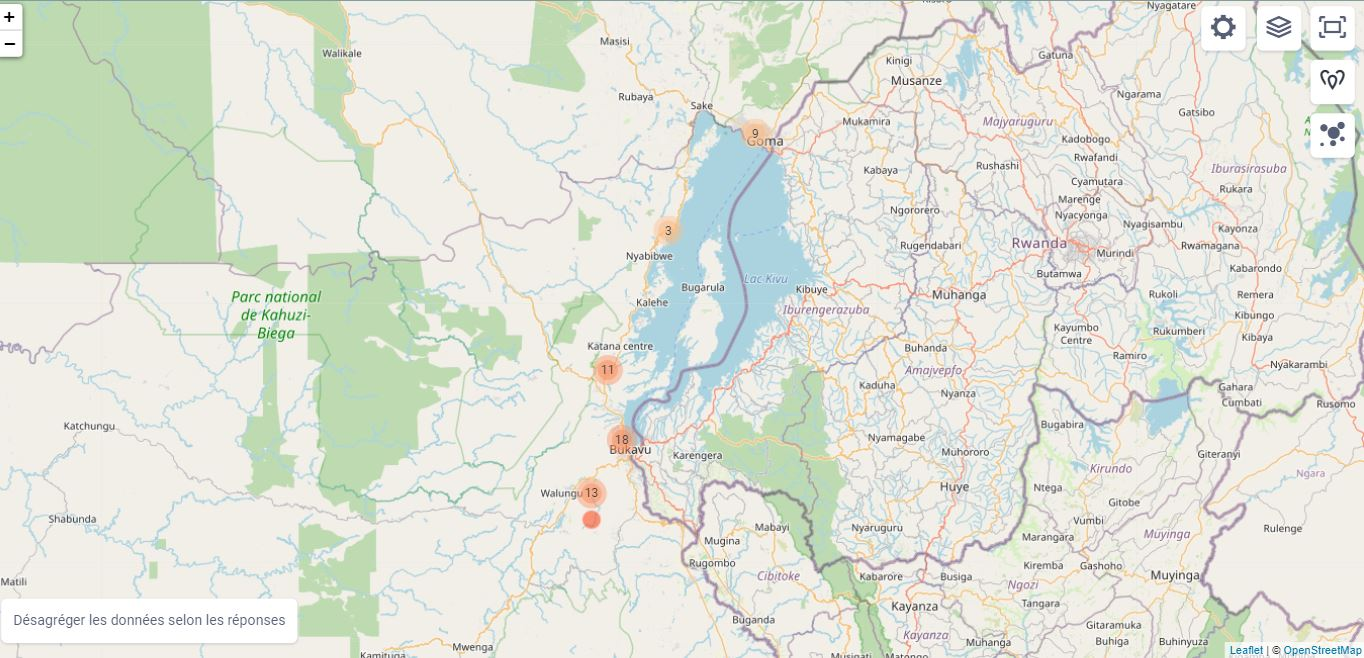
\includegraphics{Carte_enquete.JPG}
Image construite suite aux points géographiques recoltées dans l'Etude Finale sur la Cohésion Sociale du Projet SPR

\hypertarget{analyse-des-donnes}{%
\section{Analyse des donnes}\label{analyse-des-donnes}}

création de la variable durée

Analyse des durée d'enquete pour le premier Jour

\begin{verbatim}
## Adding missing grouping variables: `Territoire`
\end{verbatim}

\begin{table}

\caption{(\#tab:realisation_site)Réalisations Par Groupement et ou commune }
\centering
\begin{tabular}[t]{c|c|c|c|c|c}
\hline
\cellcolor{blue}{Province} & \cellcolor{blue}{Territoire} & \cellcolor{blue}{Territoire\_Commune} & \cellcolor{blue}{n} & \cellcolor{blue}{assignation} & \cellcolor{blue}{Pourcentage}\\
\hline
Nord-Kivu & Masisi & Masisi & 61 & 101 & 60\\
\hline
Nord-Kivu & n/a & Goma & 88 & 101 & 87\\
\hline
Sud-Kivu & Kabare & Kabare & 101 & 101 & 100\\
\hline
Sud-Kivu & Kalehe & Kalehe & 108 & 101 & 107\\
\hline
Sud-Kivu & n/a & Bukavu & 68 & 101 & 67\\
\hline
Sud-Kivu & Walungu & Walungu & 101 & 101 & 100\\
\hline
\end{tabular}
\end{table}

Temps moyen par enqueteur

\begin{verbatim}
## `summarise()` has grouped output by 'nom_enqueteur', 'Village'. You can override using the `.groups` argument.
\end{verbatim}

\begin{tabu} to \linewidth {>{\raggedright}X>{\raggedright}X>{\raggedright}X>{\raggedleft}X}
\hline
nom\_enqueteur & Village & date\_enq & temps\_moyen\\
\hline
muhindo & KALEMBERA & 2021-07-08 & 45.00000\\
\hline
agnes & n/a & 2021-07-05 & 64.16667\\
\hline
agnes & n/a & 2021-07-06 & 49.90000\\
\hline
agnes & n/a & 2021-07-07 & 44.10000\\
\hline
aziza & n/a & 2021-07-05 & 38.66667\\
\hline
aziza & n/a & 2021-07-06 & 31.41667\\
\hline
aziza & n/a & 2021-07-07 & 32.00000\\
\hline
aziza & n/a & 2021-07-08 & 38.80000\\
\hline
brigitte & KABULU I & 2021-07-05 & 33.42857\\
\hline
brigitte & KABULU I & 2021-07-06 & 151.00000\\
\hline
brigitte & KABULU II & 2021-07-07 & 36.28571\\
\hline
brigitte & NYABIBWE CENTRE & 2021-07-04 & 142.40000\\
\hline
brigitte & NYABIBWE CENTRE & 2021-07-06 & 173.80000\\
\hline
cidorho cirhulwire & CIHERANO & 2021-07-04 & 98.87500\\
\hline
cidorho cirhulwire & KAHANDA & 2021-07-06 & 43.55556\\
\hline
cidorho cirhulwire & LURHALA CENTRE & 2021-07-05 & 46.25000\\
\hline
cidorho cirhulwire & MAZIGIRO & 2021-07-07 & 44.75000\\
\hline
cikuru emmanuel & n/a & 2021-07-04 & 349.12500\\
\hline
cikuru emmanuel & n/a & 2021-07-05 & 61.18182\\
\hline
cikuru emmanuel & n/a & 2021-07-06 & 96.40000\\
\hline
cikuru emmanuel & n/a & 2021-07-07 & 56.18182\\
\hline
cikuru emmanuel & n/a & 2021-07-08 & 32.00000\\
\hline
cikuru emmanuel & n/a & 2021-07-07 & 34.00000\\
\hline
eloi zihalirwa eloi & BULOHO II & 2021-07-05 & 39.00000\\
\hline
elvis & KABULU I & 2021-07-05 & 368.00000\\
\hline
elvis & KABULU II & 2021-07-07 & 261.71429\\
\hline
gratiane hamuli & KABULU I & 2021-07-05 & 218.28571\\
\hline
gratiane hamuli & KABULU I & 2021-07-06 & 199.80000\\
\hline
gratiane hamuli & KABULU II & 2021-07-07 & 31.83333\\
\hline
gratiane hamuli & NYABIBWE CENTRE & 2021-07-04 & 160.75000\\
\hline
gratiane hamuli & NYABIBWE CENTRE & 2021-07-06 & 199.50000\\
\hline
haleine & n/a & 2021-07-05 & 55.60000\\
\hline
haleine & n/a & 2021-07-06 & 37.41667\\
\hline
haleine & n/a & 2021-07-07 & 34.63636\\
\hline
iragi & BULOHO I & 2021-07-05 & 34.66667\\
\hline
iragi & BULOHO II & 2021-07-05 & 50.66667\\
\hline
iragi & BWIMIKA & 2021-07-06 & 42.88889\\
\hline
iragi & KABALE & 2021-07-05 & 96.00000\\
\hline
iragi & KABALE & 2021-07-08 & 50.25000\\
\hline
iragi & KAMAKOMBE & 2021-07-07 & 38.75000\\
\hline
iragi & KARHANDA & 2021-07-04 & 46.50000\\
\hline
iragi & KARHANDA & 2021-07-07 & 29.00000\\
\hline
iragi olivier & BULOHO I & 2021-07-05 & 51.25000\\
\hline
iragi olivier & BULOHO II & 2021-07-05 & 40.20000\\
\hline
iragi olivier & BWIMIKA & 2021-07-06 & 39.42857\\
\hline
iragi olivier & KABALE & 2021-07-08 & 40.50000\\
\hline
iragi olivier & KAMAKOMBE & 2021-07-07 & 33.00000\\
\hline
iragi olivier & KARHANDA & 2021-07-04 & 238.00000\\
\hline
iragi olivier & KARHANDA & 2021-07-06 & 38.00000\\
\hline
iragi olivier & KARHANDA & 2021-07-07 & 39.00000\\
\hline
irene & CIHERANO & 2021-07-04 & 111.66667\\
\hline
irene & KAHANDA & 2021-07-06 & 50.77778\\
\hline
irene & LURHALA CENTRE & 2021-07-05 & 82.25000\\
\hline
irene & MAZIGIRO & 2021-07-07 & 43.00000\\
\hline
muhindo & KALEMBERA & 2021-07-08 & 42.20000\\
\hline
muhindo & KALINGA & 2021-07-06 & 43.71429\\
\hline
muhindo & TUNDA & 2021-07-08 & 42.66667\\
\hline
muhindo & WENDABANDU & 2021-07-07 & 44.28571\\
\hline
ohirwe oluhya & n/a & 2021-07-04 & 283.37500\\
\hline
ohirwe oluhya & n/a & 2021-07-05 & 45.11111\\
\hline
ohirwe oluhya & n/a & 2021-07-06 & 46.55556\\
\hline
pascal & KALEMBERA & 2021-07-08 & 46.42857\\
\hline
pascal & KALINGA & 2021-07-06 & 59.71429\\
\hline
pascal & TUNDA & 2021-07-08 & 45.66667\\
\hline
pascal & WENDABANDU & 2021-07-07 & 65.71429\\
\hline
prudent murhula & KABULU I & 2021-07-05 & 54.20000\\
\hline
prudent murhula & KABULU I & 2021-07-06 & 37.60000\\
\hline
prudent murhula & KABULU II & 2021-07-07 & 77.77778\\
\hline
prudent murhula & NYABIBWE CENTRE & 2021-07-04 & 90.84615\\
\hline
prudent murhula & NYABIBWE CENTRE & 2021-07-05 & 44.50000\\
\hline
prudent murhula & NYABIBWE CENTRE & 2021-07-06 & 37.50000\\
\hline
riziki mongane solange & CIHERANO & 2021-07-04 & 42.85714\\
\hline
riziki mongane solange & KAHANDA & 2021-07-06 & 48.37500\\
\hline
riziki mongane solange & LURHALA CENTRE & 2021-07-05 & 43.22222\\
\hline
riziki mongane solange & MAZIGIRO & 2021-07-07 & 42.66667\\
\hline
rosette & KALINGA & 2021-07-06 & 63.83333\\
\hline
rosette & KALINGA & 2021-07-07 & 57.00000\\
\hline
rosette & WENDABANDU & 2021-07-07 & 44.57143\\
\hline
rosine & BULOHO I & 2021-07-05 & 43.60000\\
\hline
rosine & BULOHO II & 2021-07-05 & 40.50000\\
\hline
rosine & BWIMIKA & 2021-07-06 & 39.77778\\
\hline
rosine & KABALE & 2021-07-08 & 49.40000\\
\hline
rosine & KAMAKOMBE & 2021-07-07 & 106.50000\\
\hline
rosine & KARHANDA & 2021-07-04 & 188.16667\\
\hline
rosine & KARHANDA & 2021-07-06 & 40.00000\\
\hline
solange riziki mongane solange & CIHERANO & 2021-07-04 & 56.00000\\
\hline
wivine & KABULU II & 2021-07-07 & 598.00000\\
\hline
wivine kababarati & KABULU II & 2021-07-07 & 41.50000\\
\hline
wivine kabarati & KABULU II & 2021-07-07 & 46.00000\\
\hline
\end{tabu}

\hypertarget{ruxe9sumuxe9-des-donnuxe9es-ruxe9coltuxe9es-duxe9sagruxe9guxe9es-selon-le-sexe-des-enquetuxe9s}{%
\section{Résumé des données récoltées désagrégées selon le sexe des enquetés}\label{ruxe9sumuxe9-des-donnuxe9es-ruxe9coltuxe9es-duxe9sagruxe9guxe9es-selon-le-sexe-des-enquetuxe9s}}

\begin{tabular}{l|l|l}
\hline
**Caractéristique** & **Femme**, N = 278 & **Homme**, N = 249\\
\hline
temps & 42 (35 – 55) & 44 (35 – 61)\\
\hline
nom\_enqueteur &  & \\
\hline
cikuru emmanuel & 23 (8·3\%) & 18 (7·2\%)\\
\hline
prudent murhula & 19 (6·8\%) & 21 (8·4\%)\\
\hline
aziza & 19 (6·8\%) & 15 (6·0\%)\\
\hline
irene & 18 (6·5\%) & 16 (6·4\%)\\
\hline
rosine & 19 (6·8\%) & 15 (6·0\%)\\
\hline
cidorho cirhulwire & 19 (6·8\%) & 14 (5·6\%)\\
\hline
iragi & 18 (6·5\%) & 15 (6·0\%)\\
\hline
iragi olivier & 19 (6·8\%) & 14 (5·6\%)\\
\hline
riziki mongane solange & 19 (6·8\%) & 14 (5·6\%)\\
\hline
brigitte & 26 (9·4\%) & 2 (0·8\%)\\
\hline
gratiane hamuli & 4 (1·4\%) & 24 (9·6\%)\\
\hline
haleine & 16 (5·8\%) & 12 (4·8\%)\\
\hline
agnes & 11 (4·0\%) & 15 (6·0\%)\\
\hline
ohirwe oluhya & 14 (5·0\%) & 12 (4·8\%)\\
\hline
pascal & 10 (3·6\%) & 14 (5·6\%)\\
\hline
muhindo & 10 (3·6\%) & 12 (4·8\%)\\
\hline
rosette & 7 (2·5\%) & 7 (2·8\%)\\
\hline
elvis & 3 (1·1\%) & 5 (2·0\%)\\
\hline
wivine kababarati & 0 (0\%) & 2 (0·8\%)\\
\hline
muhindo & 1 (0·4\%) & 0 (0\%)\\
\hline
cikuru emmanuel & 1 (0·4\%) & 0 (0\%)\\
\hline
eloi zihalirwa eloi & 0 (0\%) & 1 (0·4\%)\\
\hline
solange riziki mongane solange & 1 (0·4\%) & 0 (0\%)\\
\hline
wivine & 1 (0·4\%) & 0 (0\%)\\
\hline
wivine kabarati & 0 (0\%) & 1 (0·4\%)\\
\hline
consentement & 278 (100\%) & 249 (100\%)\\
\hline
date\_enq &  & \\
\hline
2021-07-06 & 87 (31\%) & 69 (28\%)\\
\hline
2021-07-07 & 73 (26\%) & 65 (26\%)\\
\hline
2021-07-05 & 56 (20\%) & 56 (22\%)\\
\hline
2021-07-04 & 44 (16\%) & 39 (16\%)\\
\hline
2021-07-08 & 18 (6·5\%) & 20 (8·0\%)\\
\hline
Province &  & \\
\hline
Sud-Kivu & 204 (73\%) & 174 (70\%)\\
\hline
Nord-Kivu & 74 (27\%) & 75 (30\%)\\
\hline
Ville\_territoire &  & \\
\hline
2 & 194 (70\%) & 177 (71\%)\\
\hline
1 & 84 (30\%) & 72 (29\%)\\
\hline
Ville &  & \\
\hline
n/a & 194 (70\%) & 177 (71\%)\\
\hline
1 & 46 (17\%) & 42 (17\%)\\
\hline
2 & 38 (14\%) & 30 (12\%)\\
\hline
Territoire &  & \\
\hline
n/a & 84 (30\%) & 72 (29\%)\\
\hline
Kalehe & 53 (19\%) & 55 (22\%)\\
\hline
Kabare & 56 (20\%) & 45 (18\%)\\
\hline
Walungu & 57 (21\%) & 44 (18\%)\\
\hline
Masisi & 28 (10\%) & 33 (13\%)\\
\hline
Commune &  & \\
\hline
n/a & 194 (70\%) & 177 (71\%)\\
\hline
Karisimbi & 46 (17\%) & 42 (17\%)\\
\hline
Kadutu & 38 (14\%) & 30 (12\%)\\
\hline
Quartier &  & \\
\hline
n/a & 194 (70\%) & 177 (71\%)\\
\hline
8 & 9 (3·2\%) & 9 (3·6\%)\\
\hline
5 & 10 (3·6\%) & 7 (2·8\%)\\
\hline
6 & 9 (3·2\%) & 8 (3·2\%)\\
\hline
13 & 9 (3·2\%) & 7 (2·8\%)\\
\hline
11 & 6 (2·2\%) & 9 (3·6\%)\\
\hline
10 & 10 (3·6\%) & 4 (1·6\%)\\
\hline
7 & 5 (1·8\%) & 9 (3·6\%)\\
\hline
17 & 7 (2·5\%) & 5 (2·0\%)\\
\hline
3 & 7 (2·5\%) & 5 (2·0\%)\\
\hline
12 & 6 (2·2\%) & 4 (1·6\%)\\
\hline
2 & 3 (1·1\%) & 3 (1·2\%)\\
\hline
9 & 3 (1·1\%) & 2 (0·8\%)\\
\hline
Groupement &  & \\
\hline
n/a & 84 (30\%) & 72 (29\%)\\
\hline
Mbinga Nord & 53 (19\%) & 55 (22\%)\\
\hline
Bugore & 56 (20\%) & 45 (18\%)\\
\hline
Lurhala & 57 (21\%) & 44 (18\%)\\
\hline
Biiri & 28 (10\%) & 33 (13\%)\\
\hline
Village &  & \\
\hline
n/a & 84 (30\%) & 72 (29\%)\\
\hline
NYABIBWE CENTRE & 19 (6·8\%) & 22 (8·8\%)\\
\hline
KABULU I & 17 (6·1\%) & 17 (6·8\%)\\
\hline
KABULU II & 17 (6·1\%) & 16 (6·4\%)\\
\hline
KAHANDA & 18 (6·5\%) & 8 (3·2\%)\\
\hline
BWIMIKA & 14 (5·0\%) & 11 (4·4\%)\\
\hline
CIHERANO & 13 (4·7\%) & 12 (4·8\%)\\
\hline
KARHANDA & 15 (5·4\%) & 10 (4·0\%)\\
\hline
LURHALA CENTRE & 12 (4·3\%) & 13 (5·2\%)\\
\hline
MAZIGIRO & 14 (5·0\%) & 11 (4·4\%)\\
\hline
KALINGA & 10 (3·6\%) & 11 (4·4\%)\\
\hline
WENDABANDU & 9 (3·2\%) & 12 (4·8\%)\\
\hline
KABALE & 5 (1·8\%) & 9 (3·6\%)\\
\hline
BULOHO II & 8 (2·9\%) & 5 (2·0\%)\\
\hline
KALEMBERA & 7 (2·5\%) & 6 (2·4\%)\\
\hline
BULOHO I & 6 (2·2\%) & 6 (2·4\%)\\
\hline
KAMAKOMBE & 8 (2·9\%) & 4 (1·6\%)\\
\hline
TUNDA & 2 (0·7\%) & 4 (1·6\%)\\
\hline
Tranche\_age &  & \\
\hline
1 & 174 (63\%) & 144 (58\%)\\
\hline
2 & 67 (24\%) & 61 (24\%)\\
\hline
3 & 30 (11\%) & 35 (14\%)\\
\hline
4 & 7 (2·5\%) & 9 (3·6\%)\\
\hline
Etat\_civil &  & \\
\hline
Marié(e) & 125 (45\%) & 137 (55\%)\\
\hline
Célibataire & 97 (35\%) & 94 (38\%)\\
\hline
Veuf (ve) & 28 (10\%) & 12 (4·8\%)\\
\hline
Séparé(e) & 22 (7·9\%) & 5 (2·0\%)\\
\hline
Divorcé(e) & 4 (1·4\%) & 1 (0·4\%)\\
\hline
Sans réponse & 2 (0·7\%) & 0 (0\%)\\
\hline
Margin\_group/Handicaps\_obseves/1 &  & \\
\hline
False & 66 (24\%) & 140 (56\%)\\
\hline
n/a & 74 (27\%) & 101 (41\%)\\
\hline
True & 138 (50\%) & 8 (3·2\%)\\
\hline
Margin\_group/Handicaps\_obseves/2 &  & \\
\hline
False & 182 (65\%) & 121 (49\%)\\
\hline
n/a & 74 (27\%) & 101 (41\%)\\
\hline
True & 22 (7·9\%) & 27 (11\%)\\
\hline
Margin\_group/Handicaps\_obseves/3 &  & \\
\hline
False & 203 (73\%) & 141 (57\%)\\
\hline
n/a & 74 (27\%) & 101 (41\%)\\
\hline
True & 1 (0·4\%) & 7 (2·8\%)\\
\hline
Margin\_group/Handicaps\_obseves/4 &  & \\
\hline
False & 201 (72\%) & 146 (59\%)\\
\hline
n/a & 74 (27\%) & 101 (41\%)\\
\hline
True & 3 (1·1\%) & 2 (0·8\%)\\
\hline
Margin\_group/Handicaps\_obseves/5 &  & \\
\hline
False & 202 (73\%) & 144 (58\%)\\
\hline
n/a & 74 (27\%) & 101 (41\%)\\
\hline
True & 2 (0·7\%) & 4 (1·6\%)\\
\hline
Margin\_group/Handicaps\_obseves/6 &  & \\
\hline
False & 192 (69\%) & 137 (55\%)\\
\hline
n/a & 74 (27\%) & 101 (41\%)\\
\hline
True & 12 (4·3\%) & 11 (4·4\%)\\
\hline
Margin\_group/Handicaps\_obseves/7 &  & \\
\hline
False & 202 (73\%) & 123 (49\%)\\
\hline
n/a & 74 (27\%) & 101 (41\%)\\
\hline
True & 2 (0·7\%) & 25 (10\%)\\
\hline
Margin\_group/Handicaps\_obseves/8 &  & \\
\hline
False & 173 (62\%) & 148 (59\%)\\
\hline
n/a & 74 (27\%) & 101 (41\%)\\
\hline
True & 31 (11\%) & 0 (0\%)\\
\hline
Margin\_group/Handicaps\_obseves/9 &  & \\
\hline
False & 181 (65\%) & 127 (51\%)\\
\hline
n/a & 74 (27\%) & 101 (41\%)\\
\hline
True & 23 (8·3\%) & 21 (8·4\%)\\
\hline
Margin\_group/Handicaps\_obseves/10 &  & \\
\hline
False & 200 (72\%) & 148 (59\%)\\
\hline
n/a & 74 (27\%) & 101 (41\%)\\
\hline
True & 4 (1·4\%) & 0 (0\%)\\
\hline
Margin\_group/Handicaps\_obseves/11 &  & \\
\hline
False & 186 (67\%) & 92 (37\%)\\
\hline
n/a & 74 (27\%) & 101 (41\%)\\
\hline
True & 18 (6·5\%) & 56 (22\%)\\
\hline
Margin\_group/autres\_handicaps &  & \\
\hline
n/a & 262 (94\%) & 194 (78\%)\\
\hline
Rien & 0 (0\%) & 22 (8·8\%)\\
\hline
Rien à signaler & 3 (1·1\%) & 5 (2·0\%)\\
\hline
Homme & 0 (0\%) & 5 (2·0\%)\\
\hline
Garçon & 0 (0\%) & 4 (1·6\%)\\
\hline
Fille & 3 (1·1\%) & 0 (0\%)\\
\hline
Aucun & 2 (0·7\%) & 0 (0\%)\\
\hline
Aucun handicap & 1 (0·4\%) & 1 (0·4\%)\\
\hline
Jeune garçon & 0 (0\%) & 2 (0·8\%)\\
\hline
NORMALE & 2 (0·7\%) & 0 (0\%)\\
\hline
Pas d'handicap & 0 (0\%) & 2 (0·8\%)\\
\hline
PAS D'HANDICAP & 0 (0\%) & 2 (0·8\%)\\
\hline
GARÇON & 0 (0\%) & 1 (0·4\%)\\
\hline
Garçon déplacé & 0 (0\%) & 1 (0·4\%)\\
\hline
homme & 0 (0\%) & 1 (0·4\%)\\
\hline
HOMME & 0 (0\%) & 1 (0·4\%)\\
\hline
Homme normalement & 0 (0\%) & 1 (0·4\%)\\
\hline
Jeune & 1 (0·4\%) & 0 (0\%)\\
\hline
JEUNE & 0 (0\%) & 1 (0·4\%)\\
\hline
Jeune fille & 1 (0·4\%) & 0 (0\%)\\
\hline
JEUNE FILLE & 1 (0·4\%) & 0 (0\%)\\
\hline
jeune garçon & 0 (0\%) & 1 (0·4\%)\\
\hline
Jeune garçon vulnérable & 0 (0\%) & 1 (0·4\%)\\
\hline
Jeune vulnérable & 0 (0\%) & 1 (0·4\%)\\
\hline
Pas d'hadicap & 1 (0·4\%) & 0 (0\%)\\
\hline
PAS DHANDICAP & 0 (0\%) & 1 (0·4\%)\\
\hline
PAS DHANFICAP & 0 (0\%) & 1 (0·4\%)\\
\hline
RIEN & 1 (0·4\%) & 0 (0\%)\\
\hline
Rien à indiqué & 0 (0\%) & 1 (0·4\%)\\
\hline
Niveau\_etude &  & \\
\hline
4 & 66 (24\%) & 73 (29\%)\\
\hline
1 & 72 (26\%) & 32 (13\%)\\
\hline
3 & 53 (19\%) & 45 (18\%)\\
\hline
5 & 44 (16\%) & 46 (18\%)\\
\hline
2 & 26 (9·4\%) & 18 (7·2\%)\\
\hline
6 & 13 (4·7\%) & 21 (8·4\%)\\
\hline
7 & 3 (1·1\%) & 9 (3·6\%)\\
\hline
8 & 0 (0\%) & 3 (1·2\%)\\
\hline
9 & 1 (0·4\%) & 2 (0·8\%)\\
\hline
Activite\_principale & 2·00 (1·00 – 5·00) & 3·00 (2·00 – 7·00)\\
\hline
autre\_activite &  & \\
\hline
n/a & 245 (88\%) & 202 (81\%)\\
\hline
Élève & 4 (1·4\%) & 6 (2·4\%)\\
\hline
Tailleur & 4 (1·4\%) & 1 (0·4\%)\\
\hline
COUTURIERE & 3 (1·1\%) & 0 (0\%)\\
\hline
Coiffeur & 0 (0\%) & 2 (0·8\%)\\
\hline
Couturier & 1 (0·4\%) & 1 (0·4\%)\\
\hline
Couturière & 2 (0·7\%) & 0 (0\%)\\
\hline
Eleve & 1 (0·4\%) & 1 (0·4\%)\\
\hline
Infirmier & 1 (0·4\%) & 1 (0·4\%)\\
\hline
Motard & 0 (0\%) & 2 (0·8\%)\\
\hline
Pharmacien & 0 (0\%) & 2 (0·8\%)\\
\hline
Tailleuse & 2 (0·7\%) & 0 (0\%)\\
\hline
Taximan & 0 (0\%) & 2 (0·8\%)\\
\hline
Agent de sécurité.BIFFALO & 0 (0\%) & 1 (0·4\%)\\
\hline
Ambulants & 0 (0\%) & 1 (0·4\%)\\
\hline
Aucun, mais il était infirmier avant son incapacité & 0 (0\%) & 1 (0·4\%)\\
\hline
Carellaire & 1 (0·4\%) & 0 (0\%)\\
\hline
Chauffeur & 0 (0\%) & 1 (0·4\%)\\
\hline
Chauffeur mécanicien & 0 (0\%) & 1 (0·4\%)\\
\hline
Chef de village & 0 (0\%) & 1 (0·4\%)\\
\hline
Commerce de charbon & 0 (0\%) & 1 (0·4\%)\\
\hline
Conducteur de moto & 0 (0\%) & 1 (0·4\%)\\
\hline
Coordonier & 0 (0\%) & 1 (0·4\%)\\
\hline
COORDONNIER & 0 (0\%) & 1 (0·4\%)\\
\hline
Coupe couture & 1 (0·4\%) & 0 (0\%)\\
\hline
Creuser artisanal & 0 (0\%) & 1 (0·4\%)\\
\hline
Débrouillard & 0 (0\%) & 1 (0·4\%)\\
\hline
Élève. & 0 (0\%) & 1 (0·4\%)\\
\hline
Élèves & 1 (0·4\%) & 0 (0\%)\\
\hline
Elle étudie & 1 (0·4\%) & 0 (0\%)\\
\hline
Etudiant & 0 (0\%) & 1 (0·4\%)\\
\hline
Étudiant & 1 (0·4\%) & 0 (0\%)\\
\hline
Étudiante & 1 (0·4\%) & 0 (0\%)\\
\hline
Etudie & 1 (0·4\%) & 0 (0\%)\\
\hline
EXPLOITATION MINE & 0 (0\%) & 1 (0·4\%)\\
\hline
Formation couturière & 1 (0·4\%) & 0 (0\%)\\
\hline
Je me débrouie, tout travail que je trouve,
Je le fais sans complexe. & 0 (0\%) & 1 (0·4\%)\\
\hline
Maçon & 0 (0\%) & 1 (0·4\%)\\
\hline
Maître Avocat & 0 (0\%) & 1 (0·4\%)\\
\hline
Membre de Noyon de paix de kelembera & 0 (0\%) & 1 (0·4\%)\\
\hline
menuiserie & 0 (0\%) & 1 (0·4\%)\\
\hline
Ménuisier & 0 (0\%) & 1 (0·4\%)\\
\hline
Pas d'activité, suis tout le toujours à la maison avec les enfants & 0 (0\%) & 1 (0·4\%)\\
\hline
Petit commerce & 1 (0·4\%) & 0 (0\%)\\
\hline
Petite commerçante & 1 (0·4\%) & 0 (0\%)\\
\hline
Photographe & 0 (0\%) & 1 (0·4\%)\\
\hline
Porteur des fardeaux & 0 (0\%) & 1 (0·4\%)\\
\hline
Responsable d'un petit restaurant & 1 (0·4\%) & 0 (0\%)\\
\hline
SENTINELLE & 0 (0\%) & 1 (0·4\%)\\
\hline
Soudeur et plombier & 0 (0\%) & 1 (0·4\%)\\
\hline
Suis handicapée,je ne fais rien comme travail. & 1 (0·4\%) & 0 (0\%)\\
\hline
Transporteuse des briques & 1 (0·4\%) & 0 (0\%)\\
\hline
Tresse les cheveux & 1 (0·4\%) & 0 (0\%)\\
\hline
Un gardien de sécurité & 1 (0·4\%) & 0 (0\%)\\
\hline
V unite & 0 (0\%) & 1 (0·4\%)\\
\hline
Vente unité & 0 (0\%) & 1 (0·4\%)\\
\hline
Vétérinaire & 0 (0\%) & 1 (0·4\%)\\
\hline
Duration\_milieux & 12 (5 – 25) & 15 (5 – 30)\\
\hline
relations\_entre\_personnes/Relation\_famille &  & \\
\hline
4 & 154 (55\%) & 130 (52\%)\\
\hline
5 & 85 (31\%) & 88 (35\%)\\
\hline
3 & 29 (10\%) & 22 (8·8\%)\\
\hline
2 & 8 (2·9\%) & 8 (3·2\%)\\
\hline
1 & 2 (0·7\%) & 1 (0·4\%)\\
\hline
relations\_entre\_personnes/Relation\_voisins &  & \\
\hline
4 & 154 (55\%) & 136 (55\%)\\
\hline
3 & 89 (32\%) & 75 (30\%)\\
\hline
5 & 21 (7·6\%) & 27 (11\%)\\
\hline
2 & 13 (4·7\%) & 10 (4·0\%)\\
\hline
1 & 1 (0·4\%) & 1 (0·4\%)\\
\hline
relations\_entre\_personnes/Relation\_amiscollegues\_autres\_communautaires &  & \\
\hline
4 & 158 (57\%) & 141 (57\%)\\
\hline
3 & 86 (31\%) & 70 (28\%)\\
\hline
5 & 27 (9·7\%) & 32 (13\%)\\
\hline
2 & 6 (2·2\%) & 4 (1·6\%)\\
\hline
1 & 1 (0·4\%) & 2 (0·8\%)\\
\hline
relations\_entre\_personnes/Relation\_membres\_de\_votre\_groupe\_ethnique &  & \\
\hline
4 & 147 (53\%) & 127 (51\%)\\
\hline
3 & 98 (35\%) & 94 (38\%)\\
\hline
5 & 18 (6·5\%) & 22 (8·8\%)\\
\hline
2 & 14 (5·0\%) & 6 (2·4\%)\\
\hline
1 & 1 (0·4\%) & 0 (0\%)\\
\hline
relations\_entre\_personnes/Relation\_\_autre\_groupe\_ethnique\_non\_congolais &  & \\
\hline
3 & 116 (42\%) & 111 (45\%)\\
\hline
4 & 107 (38\%) & 101 (41\%)\\
\hline
2 & 24 (8·6\%) & 15 (6·0\%)\\
\hline
1 & 25 (9·0\%) & 13 (5·2\%)\\
\hline
5 & 6 (2·2\%) & 9 (3·6\%)\\
\hline
relations\_entre\_personnes/Relation\_congolais\_autre\_groupe\_ethnique &  & \\
\hline
3 & 120 (43\%) & 118 (47\%)\\
\hline
4 & 77 (28\%) & 70 (28\%)\\
\hline
1 & 42 (15\%) & 31 (12\%)\\
\hline
2 & 35 (13\%) & 23 (9·2\%)\\
\hline
5 & 4 (1·4\%) & 7 (2·8\%)\\
\hline
Frequence\_Contact\_Congolais\_Autre\_Groupes\_Ethni &  & \\
\hline
1 & 106 (38\%) & 122 (49\%)\\
\hline
2 & 62 (22\%) & 49 (20\%)\\
\hline
4 & 68 (24\%) & 43 (17\%)\\
\hline
3 & 23 (8·3\%) & 23 (9·2\%)\\
\hline
5 & 19 (6·8\%) & 12 (4·8\%)\\
\hline
Participation\_Ensemble/Freq\_Part\_Ceremonie\_Culturelle &  & \\
\hline
2 & 65 (23\%) & 79 (32\%)\\
\hline
4 & 82 (29\%) & 60 (24\%)\\
\hline
1 & 58 (21\%) & 52 (21\%)\\
\hline
3 & 53 (19\%) & 41 (16\%)\\
\hline
5 & 20 (7·2\%) & 17 (6·8\%)\\
\hline
Participation\_Ensemble/Freq\_Part\_Meme\_Eglise &  & \\
\hline
2 & 108 (39\%) & 94 (38\%)\\
\hline
1 & 78 (28\%) & 74 (30\%)\\
\hline
4 & 59 (21\%) & 46 (18\%)\\
\hline
3 & 17 (6·1\%) & 21 (8·4\%)\\
\hline
5 & 16 (5·8\%) & 14 (5·6\%)\\
\hline
Participation\_Ensemble/Freq\_Part\_Travail\_Ensemble &  & \\
\hline
1 & 97 (35\%) & 108 (43\%)\\
\hline
4 & 79 (28\%) & 62 (25\%)\\
\hline
2 & 52 (19\%) & 43 (17\%)\\
\hline
5 & 26 (9·4\%) & 18 (7·2\%)\\
\hline
3 & 24 (8·6\%) & 18 (7·2\%)\\
\hline
Participation\_Ensemble/Freq\_Mariage\_InterEthnique &  & \\
\hline
4 & 72 (26\%) & 53 (21\%)\\
\hline
2 & 53 (19\%) & 54 (22\%)\\
\hline
3 & 58 (21\%) & 48 (19\%)\\
\hline
1 & 52 (19\%) & 44 (18\%)\\
\hline
5 & 43 (15\%) & 50 (20\%)\\
\hline
DIM1\_4\_1 &  & \\
\hline
1 & 133 (48\%) & 124 (50\%)\\
\hline
2 & 87 (31\%) & 81 (33\%)\\
\hline
4 & 35 (13\%) & 28 (11\%)\\
\hline
3 & 23 (8·3\%) & 16 (6·4\%)\\
\hline
DIM1\_4\_2 &  & \\
\hline
1 & 154 (55\%) & 133 (53\%)\\
\hline
2 & 68 (24\%) & 65 (26\%)\\
\hline
4 & 43 (15\%) & 32 (13\%)\\
\hline
3 & 13 (4·7\%) & 19 (7·6\%)\\
\hline
DIM1\_4\_3 &  & \\
\hline
1 & 133 (48\%) & 126 (51\%)\\
\hline
2 & 90 (32\%) & 71 (29\%)\\
\hline
4 & 29 (10\%) & 27 (11\%)\\
\hline
3 & 26 (9·4\%) & 25 (10\%)\\
\hline
DIM1\_4\_4 &  & \\
\hline
1 & 154 (55\%) & 136 (55\%)\\
\hline
2 & 66 (24\%) & 61 (24\%)\\
\hline
4 & 38 (14\%) & 30 (12\%)\\
\hline
3 & 20 (7·2\%) & 22 (8·8\%)\\
\hline
DIM1\_5\_1 &  & \\
\hline
1 & 133 (48\%) & 118 (47\%)\\
\hline
2 & 65 (23\%) & 62 (25\%)\\
\hline
4 & 57 (21\%) & 44 (18\%)\\
\hline
3 & 23 (8·3\%) & 25 (10\%)\\
\hline
DIM1\_5\_2 &  & \\
\hline
1 & 149 (54\%) & 126 (51\%)\\
\hline
4 & 67 (24\%) & 49 (20\%)\\
\hline
2 & 47 (17\%) & 53 (21\%)\\
\hline
3 & 15 (5·4\%) & 21 (8·4\%)\\
\hline
DIM1\_5\_3 &  & \\
\hline
1 & 122 (44\%) & 106 (43\%)\\
\hline
2 & 69 (25\%) & 73 (29\%)\\
\hline
4 & 55 (20\%) & 40 (16\%)\\
\hline
3 & 32 (12\%) & 30 (12\%)\\
\hline
DIM1\_5\_4 &  & \\
\hline
1 & 133 (48\%) & 126 (51\%)\\
\hline
2 & 56 (20\%) & 55 (22\%)\\
\hline
4 & 60 (22\%) & 42 (17\%)\\
\hline
3 & 29 (10\%) & 26 (10\%)\\
\hline
DIM1\_6 &  & \\
\hline
3 & 92 (33\%) & 74 (30\%)\\
\hline
2 & 81 (29\%) & 80 (32\%)\\
\hline
1 & 66 (24\%) & 74 (30\%)\\
\hline
4 & 39 (14\%) & 21 (8·4\%)\\
\hline
DIM1\_7/1 & 78 (28\%) & 78 (31\%)\\
\hline
DIM1\_7/2 & 127 (46\%) & 104 (42\%)\\
\hline
DIM1\_7/3 & 75 (27\%) & 89 (36\%)\\
\hline
DIM1\_7/4 & 77 (28\%) & 75 (30\%)\\
\hline
DIM1\_7/5 & 69 (25\%) & 65 (26\%)\\
\hline
DIM1\_7/6 & 33 (12\%) & 31 (12\%)\\
\hline
DIM1\_7/7 & 34 (12\%) & 30 (12\%)\\
\hline
DIM1\_7/8 & 43 (15\%) & 57 (23\%)\\
\hline
DIM1\_7/9 & 77 (28\%) & 78 (31\%)\\
\hline
DIM1\_7/10 & 22 (7·9\%) & 9 (3·6\%)\\
\hline
DIM1\_7/11 & 7 (2·5\%) & 6 (2·4\%)\\
\hline
DIM1\_7/12 & 14 (5·0\%) & 6 (2·4\%)\\
\hline
DIM1\_7a &  & \\
\hline
n/a & 267 (96\%) & 245 (98\%)\\
\hline
Ils ne sont pas ici & 2 (0·7\%) & 0 (0\%)\\
\hline
Avoir les leaders qui peuvent plaider pour nous & 1 (0·4\%) & 0 (0\%)\\
\hline
Changement de mentalité & 1 (0·4\%) & 0 (0\%)\\
\hline
Changer la mentalité des autorités & 0 (0\%) & 1 (0·4\%)\\
\hline
IL FAUT QU'IL Y EST LA PAIX POUR QUE CHAQUE PEUPLE REGAGNE SON MILIEU D'ORIGINE & 1 (0·4\%) & 0 (0\%)\\
\hline
Ils ne sont pas chez nous & 1 (0·4\%) & 0 (0\%)\\
\hline
Ils ne sont pas ici chez nous & 1 (0·4\%) & 0 (0\%)\\
\hline
Je ne sais rien. Nous ne sommes que bashi ici & 1 (0·4\%) & 0 (0\%)\\
\hline
Le fait être sédentaire & 0 (0\%) & 1 (0·4\%)\\
\hline
Ne pas les accueillir & 0 (0\%) & 1 (0·4\%)\\
\hline
Nous sommes seulement des shi & 1 (0·4\%) & 0 (0\%)\\
\hline
Pas de gens d'autre tribub ici & 0 (0\%) & 1 (0·4\%)\\
\hline
Prôner l'amour & 1 (0·4\%) & 0 (0\%)\\
\hline
S'ASSOIR EN ENSEMBLE & 1 (0·4\%) & 0 (0\%)\\
\hline
2/DIM2\_1/A &  & \\
\hline
True & 144 (52\%) & 134 (54\%)\\
\hline
False & 129 (46\%) & 110 (44\%)\\
\hline
n/a & 5 (1·8\%) & 5 (2·0\%)\\
\hline
2/DIM2\_1/B &  & \\
\hline
True & 173 (62\%) & 159 (64\%)\\
\hline
False & 100 (36\%) & 85 (34\%)\\
\hline
n/a & 5 (1·8\%) & 5 (2·0\%)\\
\hline
2/DIM2\_1/C &  & \\
\hline
False & 168 (60\%) & 126 (51\%)\\
\hline
True & 105 (38\%) & 118 (47\%)\\
\hline
n/a & 5 (1·8\%) & 5 (2·0\%)\\
\hline
2/DIM2\_1/D &  & \\
\hline
False & 159 (57\%) & 161 (65\%)\\
\hline
True & 114 (41\%) & 83 (33\%)\\
\hline
n/a & 5 (1·8\%) & 5 (2·0\%)\\
\hline
2/DIM2\_1/E &  & \\
\hline
False & 236 (85\%) & 208 (84\%)\\
\hline
True & 37 (13\%) & 36 (14\%)\\
\hline
n/a & 5 (1·8\%) & 5 (2·0\%)\\
\hline
2/DIM2\_1/F &  & \\
\hline
False & 204 (73\%) & 168 (67\%)\\
\hline
True & 69 (25\%) & 76 (31\%)\\
\hline
n/a & 5 (1·8\%) & 5 (2·0\%)\\
\hline
2/DIM2\_1/G &  & \\
\hline
False & 184 (66\%) & 175 (70\%)\\
\hline
True & 89 (32\%) & 69 (28\%)\\
\hline
n/a & 5 (1·8\%) & 5 (2·0\%)\\
\hline
2/DIM2\_1/H &  & \\
\hline
False & 203 (73\%) & 190 (76\%)\\
\hline
True & 70 (25\%) & 54 (22\%)\\
\hline
n/a & 5 (1·8\%) & 5 (2·0\%)\\
\hline
2/DIM2\_1/I &  & \\
\hline
False & 193 (69\%) & 177 (71\%)\\
\hline
True & 80 (29\%) & 67 (27\%)\\
\hline
n/a & 5 (1·8\%) & 5 (2·0\%)\\
\hline
2/DIM2\_1/J &  & \\
\hline
False & 213 (77\%) & 198 (80\%)\\
\hline
True & 60 (22\%) & 46 (18\%)\\
\hline
n/a & 5 (1·8\%) & 5 (2·0\%)\\
\hline
2/DIM2\_1/K &  & \\
\hline
False & 189 (68\%) & 172 (69\%)\\
\hline
True & 84 (30\%) & 72 (29\%)\\
\hline
n/a & 5 (1·8\%) & 5 (2·0\%)\\
\hline
2/DIM2\_2/DIM2\_2\_1 &  & \\
\hline
3 & 121 (44\%) & 95 (38\%)\\
\hline
4 & 89 (32\%) & 87 (35\%)\\
\hline
2 & 44 (16\%) & 44 (18\%)\\
\hline
1 & 16 (5·8\%) & 15 (6·0\%)\\
\hline
5 & 8 (2·9\%) & 8 (3·2\%)\\
\hline
2/DIM2\_2/DIM2\_2\_2 &  & \\
\hline
3 & 146 (53\%) & 118 (47\%)\\
\hline
4 & 73 (26\%) & 67 (27\%)\\
\hline
2 & 36 (13\%) & 35 (14\%)\\
\hline
1 & 22 (7·9\%) & 20 (8·0\%)\\
\hline
5 & 1 (0·4\%) & 9 (3·6\%)\\
\hline
2/DIM2\_2/DIM2\_2\_3 &  & \\
\hline
3 & 104 (37\%) & 106 (43\%)\\
\hline
1 & 75 (27\%) & 62 (25\%)\\
\hline
2 & 68 (24\%) & 55 (22\%)\\
\hline
4 & 30 (11\%) & 22 (8·8\%)\\
\hline
5 & 1 (0·4\%) & 4 (1·6\%)\\
\hline
2/DIM2\_2/DIM2\_2\_4 &  & \\
\hline
1 & 122 (44\%) & 101 (41\%)\\
\hline
2 & 77 (28\%) & 69 (28\%)\\
\hline
3 & 66 (24\%) & 62 (25\%)\\
\hline
4 & 12 (4·3\%) & 14 (5·6\%)\\
\hline
5 & 1 (0·4\%) & 3 (1·2\%)\\
\hline
2/DIM2\_3/a & 82 (29\%) & 89 (36\%)\\
\hline
2/DIM2\_3/b & 90 (32\%) & 82 (33\%)\\
\hline
2/DIM2\_3/c & 129 (46\%) & 97 (39\%)\\
\hline
2/DIM2\_3/d & 104 (37\%) & 71 (29\%)\\
\hline
2/DIM2\_3/e & 83 (30\%) & 78 (31\%)\\
\hline
2/DIM2\_3/f & 54 (19\%) & 62 (25\%)\\
\hline
2/DIM2\_3/g & 64 (23\%) & 64 (26\%)\\
\hline
2/DIM2\_3/h & 3 (1·1\%) & 4 (1·6\%)\\
\hline
2/DIM2\_3/i & 11 (4·0\%) & 6 (2·4\%)\\
\hline
2/DIM2\_3/j & 43 (15\%) & 37 (15\%)\\
\hline
2/DIM2\_3/k & 21 (7·6\%) & 15 (6·0\%)\\
\hline
2/DIM2\_3/l & 5 (1·8\%) & 8 (3·2\%)\\
\hline
2/DIM2\_3a &  & \\
\hline
n/a & 273 (98\%) & 241 (97\%)\\
\hline
Arrêt des conflits & 1 (0·4\%) & 0 (0\%)\\
\hline
Ces gens ne sont pas ici & 0 (0\%) & 1 (0·4\%)\\
\hline
Des loisirs entre eux & 0 (0\%) & 1 (0·4\%)\\
\hline
Éviter les jalousies & 1 (0·4\%) & 0 (0\%)\\
\hline
il faut éradiquer le tribalisme & 0 (0\%) & 1 (0·4\%)\\
\hline
Il faut qu'il y ait pacte de sang. & 0 (0\%) & 1 (0·4\%)\\
\hline
Il faut que les tribus se pardonnent. & 1 (0·4\%) & 0 (0\%)\\
\hline
Il n'y a pas d'autres groupes ethniques ! & 1 (0·4\%) & 0 (0\%)\\
\hline
Integegration des toutes les couches dans toutes les activite sans distinction encourager le mariage avec d'autres tribut non congolais & 0 (0\%) & 1 (0·4\%)\\
\hline
Le respect de tout un  chacun & 0 (0\%) & 1 (0·4\%)\\
\hline
Mettre en place des groupes des discussions & 1 (0·4\%) & 0 (0\%)\\
\hline
Se marier dans différents groupes ethniques & 0 (0\%) & 1 (0·4\%)\\
\hline
Sensibilisation, faire de théâtre pour montrer l'importance de vivre ensemble & 0 (0\%) & 1 (0·4\%)\\
\hline
2/DIM2\_4 &  & \\
\hline
4 & 109 (39\%) & 109 (44\%)\\
\hline
3 & 78 (28\%) & 72 (29\%)\\
\hline
5 & 65 (23\%) & 50 (20\%)\\
\hline
2 & 25 (9·0\%) & 15 (6·0\%)\\
\hline
1 & 1 (0·4\%) & 3 (1·2\%)\\
\hline
2/DIM2\_5 &  & \\
\hline
3 & 131 (47\%) & 124 (50\%)\\
\hline
2 & 66 (24\%) & 60 (24\%)\\
\hline
4 & 65 (23\%) & 51 (20\%)\\
\hline
1 & 12 (4·3\%) & 9 (3·6\%)\\
\hline
5 & 4 (1·4\%) & 5 (2·0\%)\\
\hline
2/DIM2\_6 &  & \\
\hline
3 & 153 (55\%) & 136 (55\%)\\
\hline
2 & 56 (20\%) & 54 (22\%)\\
\hline
4 & 51 (18\%) & 44 (18\%)\\
\hline
1 & 12 (4·3\%) & 9 (3·6\%)\\
\hline
5 & 6 (2·2\%) & 6 (2·4\%)\\
\hline
2/DIM2\_7 &  & \\
\hline
3 & 111 (40\%) & 112 (45\%)\\
\hline
2 & 107 (38\%) & 89 (36\%)\\
\hline
1 & 34 (12\%) & 23 (9·2\%)\\
\hline
4 & 25 (9·0\%) & 24 (9·6\%)\\
\hline
5 & 1 (0·4\%) & 1 (0·4\%)\\
\hline
2/DIM2\_8 &  & \\
\hline
2 & 112 (40\%) & 102 (41\%)\\
\hline
3 & 74 (27\%) & 67 (27\%)\\
\hline
1 & 73 (26\%) & 66 (27\%)\\
\hline
4 & 17 (6·1\%) & 14 (5·6\%)\\
\hline
5 & 2 (0·7\%) & 0 (0\%)\\
\hline
2/DIM2\_9/a & 40 (14\%) & 36 (14\%)\\
\hline
2/DIM2\_9/b & 98 (35\%) & 92 (37\%)\\
\hline
2/DIM2\_9/c & 53 (19\%) & 65 (26\%)\\
\hline
2/DIM2\_9/d & 54 (19\%) & 50 (20\%)\\
\hline
2/DIM2\_9/e & 73 (26\%) & 57 (23\%)\\
\hline
2/DIM2\_9/f & 58 (21\%) & 44 (18\%)\\
\hline
2/DIM2\_9/g & 35 (13\%) & 37 (15\%)\\
\hline
2/DIM2\_9/h & 20 (7·2\%) & 19 (7·6\%)\\
\hline
2/DIM2\_9/i & 16 (5·8\%) & 24 (9·6\%)\\
\hline
2/DIM2\_9/j & 36 (13\%) & 31 (12\%)\\
\hline
2/DIM2\_9/k & 13 (4·7\%) & 10 (4·0\%)\\
\hline
2/DIM2\_9/l & 5 (1·8\%) & 1 (0·4\%)\\
\hline
2/DIM2\_9/m & 30 (11\%) & 24 (9·6\%)\\
\hline
2/DIM2\_9/n & 4 (1·4\%) & 2 (0·8\%)\\
\hline
2/DIM2\_9/o & 17 (6·1\%) & 5 (2·0\%)\\
\hline
2/DIM2\_9/p & 5 (1·8\%) & 4 (1·6\%)\\
\hline
2/DIM2\_9a &  & \\
\hline
n/a & 273 (98\%) & 245 (98\%)\\
\hline
Cesser de faire du mal & 0 (0\%) & 1 (0·4\%)\\
\hline
Chez nous il n'y a pas d'autres groupes ethniques & 1 (0·4\%) & 0 (0\%)\\
\hline
Créer de bonne relation & 0 (0\%) & 1 (0·4\%)\\
\hline
Créer Les conditions de la paix durable & 1 (0·4\%) & 0 (0\%)\\
\hline
Éviter de soupçons & 1 (0·4\%) & 0 (0\%)\\
\hline
Faire de mixages dans les services étatiques et privés et financer les associations locales pour sensibiliser la communauté locale à la cohabitation pacifique. Voire les hutu,les guides,les tutsi & 0 (0\%) & 1 (0·4\%)\\
\hline
L' entraides & 1 (0·4\%) & 0 (0\%)\\
\hline
L'amour & 0 (0\%) & 1 (0·4\%)\\
\hline
LA CONFIANCE POUR MOI NEST PAS TRES FACILE & 1 (0·4\%) & 0 (0\%)\\
\hline
3/DIM3\_1/DIM3\_1\_1 &  & \\
\hline
3 & 111 (40\%) & 85 (34\%)\\
\hline
4 & 81 (29\%) & 71 (29\%)\\
\hline
2 & 63 (23\%) & 68 (27\%)\\
\hline
1 & 17 (6·1\%) & 18 (7·2\%)\\
\hline
5 & 6 (2·2\%) & 7 (2·8\%)\\
\hline
3/DIM3\_1/DIM3\_1\_2 &  & \\
\hline
3 & 125 (45\%) & 92 (37\%)\\
\hline
2 & 82 (29\%) & 69 (28\%)\\
\hline
4 & 49 (18\%) & 61 (24\%)\\
\hline
1 & 19 (6·8\%) & 21 (8·4\%)\\
\hline
5 & 3 (1·1\%) & 6 (2·4\%)\\
\hline
3/DIM3\_1/DIM3\_1\_3 &  & \\
\hline
2 & 106 (38\%) & 87 (35\%)\\
\hline
3 & 87 (31\%) & 70 (28\%)\\
\hline
4 & 49 (18\%) & 55 (22\%)\\
\hline
1 & 33 (12\%) & 30 (12\%)\\
\hline
5 & 3 (1·1\%) & 7 (2·8\%)\\
\hline
3/DIM3\_1/DIM3\_1\_4 &  & \\
\hline
2 & 105 (38\%) & 90 (36\%)\\
\hline
3 & 79 (28\%) & 63 (25\%)\\
\hline
1 & 62 (22\%) & 54 (22\%)\\
\hline
4 & 31 (11\%) & 40 (16\%)\\
\hline
5 & 1 (0·4\%) & 2 (0·8\%)\\
\hline
3/DIM3\_1/DIM3\_1\_5 &  & \\
\hline
1 & 104 (37\%) & 93 (37\%)\\
\hline
2 & 99 (36\%) & 90 (36\%)\\
\hline
3 & 56 (20\%) & 46 (18\%)\\
\hline
4 & 18 (6·5\%) & 19 (7·6\%)\\
\hline
5 & 1 (0·4\%) & 1 (0·4\%)\\
\hline
3/DIM3\_1/DIM3\_1\_6 &  & \\
\hline
1 & 118 (42\%) & 101 (41\%)\\
\hline
2 & 100 (36\%) & 89 (36\%)\\
\hline
3 & 44 (16\%) & 42 (17\%)\\
\hline
4 & 15 (5·4\%) & 17 (6·8\%)\\
\hline
5 & 1 (0·4\%) & 0 (0\%)\\
\hline
3/DIM3\_1/DIM3\_1\_7 &  & \\
\hline
3 & 110 (40\%) & 102 (41\%)\\
\hline
4 & 90 (32\%) & 83 (33\%)\\
\hline
2 & 53 (19\%) & 40 (16\%)\\
\hline
1 & 14 (5·0\%) & 14 (5·6\%)\\
\hline
5 & 11 (4·0\%) & 10 (4·0\%)\\
\hline
3/DIM3\_1/DIM3\_1\_8 &  & \\
\hline
4 & 117 (42\%) & 99 (40\%)\\
\hline
3 & 67 (24\%) & 68 (27\%)\\
\hline
5 & 63 (23\%) & 53 (21\%)\\
\hline
2 & 26 (9·4\%) & 22 (8·8\%)\\
\hline
1 & 5 (1·8\%) & 7 (2·8\%)\\
\hline
3/DIM3\_1/DIM3\_1\_9 &  & \\
\hline
3 & 139 (50\%) & 110 (44\%)\\
\hline
4 & 58 (21\%) & 71 (29\%)\\
\hline
2 & 49 (18\%) & 39 (16\%)\\
\hline
1 & 21 (7·6\%) & 21 (8·4\%)\\
\hline
5 & 11 (4·0\%) & 8 (3·2\%)\\
\hline
3/DIM3\_1/DIM3\_1\_10 &  & \\
\hline
3 & 123 (44\%) & 94 (38\%)\\
\hline
4 & 56 (20\%) & 71 (29\%)\\
\hline
2 & 58 (21\%) & 53 (21\%)\\
\hline
1 & 36 (13\%) & 26 (10\%)\\
\hline
5 & 5 (1·8\%) & 5 (2·0\%)\\
\hline
3/DIM3\_1/DIM3\_1\_11 &  & \\
\hline
3 & 97 (35\%) & 69 (28\%)\\
\hline
2 & 86 (31\%) & 79 (32\%)\\
\hline
1 & 77 (28\%) & 70 (28\%)\\
\hline
4 & 15 (5·4\%) & 30 (12\%)\\
\hline
5 & 3 (1·1\%) & 1 (0·4\%)\\
\hline
3/DIM3\_2/a & 133 (48\%) & 127 (51\%)\\
\hline
3/DIM3\_2/b & 75 (27\%) & 97 (39\%)\\
\hline
3/DIM3\_2/c & 128 (46\%) & 116 (47\%)\\
\hline
3/DIM3\_2/d & 54 (19\%) & 46 (18\%)\\
\hline
3/DIM3\_2/e & 95 (34\%) & 72 (29\%)\\
\hline
3/DIM3\_2/f & 101 (36\%) & 75 (30\%)\\
\hline
3/DIM3\_2/g & 22 (7·9\%) & 33 (13\%)\\
\hline
3/DIM3\_2/h & 58 (21\%) & 41 (16\%)\\
\hline
3/DIM3\_2/i & 6 (2·2\%) & 6 (2·4\%)\\
\hline
3/DIM3\_2/j & 1 (0·4\%) & 1 (0·4\%)\\
\hline
3/DIM3\_2/k & 13 (4·7\%) & 12 (4·8\%)\\
\hline
3/DIM3\_2a &  & \\
\hline
n/a & 265 (95\%) & 237 (95\%)\\
\hline
Aider la population & 1 (0·4\%) & 0 (0\%)\\
\hline
AIMER TOUT LE MONDE AU MÊME POINT D'ÉGALITÉ & 0 (0\%) & 1 (0·4\%)\\
\hline
Autorité ayant le soucis de la population & 1 (0·4\%) & 0 (0\%)\\
\hline
Considération  egale & 0 (0\%) & 1 (0·4\%)\\
\hline
Des autorités conscientes & 0 (0\%) & 1 (0·4\%)\\
\hline
DES NON TRIBAL & 1 (0·4\%) & 0 (0\%)\\
\hline
Développement & 0 (0\%) & 1 (0·4\%)\\
\hline
Être proche de la population & 0 (0\%) & 1 (0·4\%)\\
\hline
ÊTRE SOCIAL ET SAVOIR COMMUNIQUER AVEC LES GENS & 1 (0·4\%) & 0 (0\%)\\
\hline
Éviter la discrimination et la haine envers la population & 0 (0\%) & 1 (0·4\%)\\
\hline
Formation de tous les chefs & 1 (0·4\%) & 0 (0\%)\\
\hline
Il faut éradiquer l'impunité. & 0 (0\%) & 1 (0·4\%)\\
\hline
Il faut nous soyons sécurisé & 1 (0·4\%) & 0 (0\%)\\
\hline
Les chefs doivent être impartiaux & 1 (0·4\%) & 0 (0\%)\\
\hline
Lutter pour la paix , Éviter la discrimination & 1 (0·4\%) & 0 (0\%)\\
\hline
Nous donner un bon travail, valoriser nos diplômes & 1 (0·4\%) & 0 (0\%)\\
\hline
Nous donner un élevage & 0 (0\%) & 1 (0·4\%)\\
\hline
On doit oublier le passé & 0 (0\%) & 1 (0·4\%)\\
\hline
Prendre en charges les  démobilisé. & 0 (0\%) & 1 (0·4\%)\\
\hline
QU'ILS SOIENT UNIS ET COLLABORANTS & 1 (0·4\%) & 0 (0\%)\\
\hline
Que les autorités nous aiment comme leurs propres enfants & 1 (0·4\%) & 0 (0\%)\\
\hline
QUILS SE RESPECTENT EUX MEME D'ABORD & 1 (0·4\%) & 0 (0\%)\\
\hline
Renforcer en capacité nos autorités & 0 (0\%) & 1 (0·4\%)\\
\hline
Sensibilisation, rapprochement de la population & 0 (0\%) & 1 (0·4\%)\\
\hline
Sensibiliser toute la communauté à la cohésion sociale & 1 (0·4\%) & 0 (0\%)\\
\hline
4/DIM4\_1/DIM4\_1\_1 &  & \\
\hline
2 & 107 (38\%) & 90 (36\%)\\
\hline
4 & 75 (27\%) & 86 (35\%)\\
\hline
3 & 40 (14\%) & 38 (15\%)\\
\hline
1 & 33 (12\%) & 20 (8·0\%)\\
\hline
5 & 23 (8·3\%) & 15 (6·0\%)\\
\hline
4/DIM4\_1/DIM4\_1\_2 &  & \\
\hline
2 & 130 (47\%) & 119 (48\%)\\
\hline
3 & 59 (21\%) & 50 (20\%)\\
\hline
4 & 42 (15\%) & 52 (21\%)\\
\hline
1 & 43 (15\%) & 23 (9·2\%)\\
\hline
5 & 4 (1·4\%) & 5 (2·0\%)\\
\hline
4/DIM4\_1/DIM4\_1\_3 &  & \\
\hline
2 & 98 (35\%) & 91 (37\%)\\
\hline
4 & 78 (28\%) & 79 (32\%)\\
\hline
3 & 64 (23\%) & 54 (22\%)\\
\hline
1 & 32 (12\%) & 21 (8·4\%)\\
\hline
5 & 6 (2·2\%) & 4 (1·6\%)\\
\hline
4/DIM4\_1/DIM4\_1\_4 &  & \\
\hline
4 & 102 (37\%) & 106 (43\%)\\
\hline
2 & 83 (30\%) & 72 (29\%)\\
\hline
3 & 62 (22\%) & 57 (23\%)\\
\hline
1 & 22 (7·9\%) & 12 (4·8\%)\\
\hline
5 & 9 (3·2\%) & 2 (0·8\%)\\
\hline
4/DIM4\_1/DIM4\_1\_5 &  & \\
\hline
4 & 143 (51\%) & 142 (57\%)\\
\hline
2 & 55 (20\%) & 42 (17\%)\\
\hline
3 & 39 (14\%) & 40 (16\%)\\
\hline
5 & 30 (11\%) & 16 (6·4\%)\\
\hline
1 & 11 (4·0\%) & 9 (3·6\%)\\
\hline
4/DIM4\_1/DIM4\_1\_6 &  & \\
\hline
2 & 125 (45\%) & 117 (47\%)\\
\hline
1 & 72 (26\%) & 48 (19\%)\\
\hline
3 & 43 (15\%) & 47 (19\%)\\
\hline
4 & 36 (13\%) & 34 (14\%)\\
\hline
5 & 2 (0·7\%) & 3 (1·2\%)\\
\hline
4/DIM4\_1/DIM4\_1\_7 &  & \\
\hline
4 & 129 (46\%) & 117 (47\%)\\
\hline
3 & 63 (23\%) & 49 (20\%)\\
\hline
2 & 51 (18\%) & 54 (22\%)\\
\hline
5 & 17 (6·1\%) & 21 (8·4\%)\\
\hline
1 & 18 (6·5\%) & 8 (3·2\%)\\
\hline
4/DIM4\_1/DIM4\_1\_8 &  & \\
\hline
2 & 112 (40\%) & 101 (41\%)\\
\hline
3 & 67 (24\%) & 54 (22\%)\\
\hline
1 & 62 (22\%) & 43 (17\%)\\
\hline
4 & 35 (13\%) & 46 (18\%)\\
\hline
5 & 2 (0·7\%) & 5 (2·0\%)\\
\hline
5/DIM5\_1 &  & \\
\hline
1 & 156 (56\%) & 133 (53\%)\\
\hline
2 & 88 (32\%) & 87 (35\%)\\
\hline
3 & 34 (12\%) & 29 (12\%)\\
\hline
5/DIM5\_2 &  & \\
\hline
3 & 70 (25\%) & 84 (34\%)\\
\hline
2 & 78 (28\%) & 55 (22\%)\\
\hline
1 & 66 (24\%) & 54 (22\%)\\
\hline
4 & 38 (14\%) & 29 (12\%)\\
\hline
99 & 17 (6·1\%) & 10 (4·0\%)\\
\hline
5 & 9 (3·2\%) & 16 (6·4\%)\\
\hline
999 & 0 (0\%) & 1 (0·4\%)\\
\hline
5/DIM5\_3 &  & \\
\hline
4 & 94 (34\%) & 81 (33\%)\\
\hline
3 & 65 (23\%) & 63 (25\%)\\
\hline
5 & 54 (19\%) & 48 (19\%)\\
\hline
2 & 30 (11\%) & 28 (11\%)\\
\hline
99 & 25 (9·0\%) & 23 (9·2\%)\\
\hline
1 & 8 (2·9\%) & 6 (2·4\%)\\
\hline
999 & 2 (0·7\%) & 0 (0\%)\\
\hline
5/DIM5\_4 &  & \\
\hline
3 & 93 (33\%) & 90 (36\%)\\
\hline
4 & 81 (29\%) & 59 (24\%)\\
\hline
2 & 62 (22\%) & 60 (24\%)\\
\hline
5 & 28 (10\%) & 24 (9·6\%)\\
\hline
1 & 13 (4·7\%) & 8 (3·2\%)\\
\hline
99 & 1 (0·4\%) & 8 (3·2\%)\\
\hline
5/DIM5\_5 &  & \\
\hline
2 & 84 (30\%) & 64 (26\%)\\
\hline
3 & 70 (25\%) & 61 (24\%)\\
\hline
1 & 45 (16\%) & 37 (15\%)\\
\hline
4 & 39 (14\%) & 43 (17\%)\\
\hline
5 & 27 (9·7\%) & 31 (12\%)\\
\hline
99 & 13 (4·7\%) & 12 (4·8\%)\\
\hline
999 & 0 (0\%) & 1 (0·4\%)\\
\hline
5/DIM5\_6 &  & \\
\hline
3 & 109 (39\%) & 92 (37\%)\\
\hline
2 & 76 (27\%) & 71 (29\%)\\
\hline
4 & 52 (19\%) & 41 (16\%)\\
\hline
1 & 27 (9·7\%) & 24 (9·6\%)\\
\hline
5 & 11 (4·0\%) & 20 (8·0\%)\\
\hline
99 & 3 (1·1\%) & 1 (0·4\%)\\
\hline
5/DIM5\_7 &  & \\
\hline
4 & 89 (32\%) & 80 (32\%)\\
\hline
5 & 80 (29\%) & 66 (27\%)\\
\hline
3 & 53 (19\%) & 60 (24\%)\\
\hline
2 & 40 (14\%) & 31 (12\%)\\
\hline
1 & 14 (5·0\%) & 10 (4·0\%)\\
\hline
99 & 2 (0·7\%) & 2 (0·8\%)\\
\hline
5/DIM5\_8 &  & \\
\hline
2 & 122 (44\%) & 101 (41\%)\\
\hline
1 & 63 (23\%) & 53 (21\%)\\
\hline
3 & 51 (18\%) & 43 (17\%)\\
\hline
4 & 26 (9·4\%) & 27 (11\%)\\
\hline
5 & 6 (2·2\%) & 18 (7·2\%)\\
\hline
99 & 9 (3·2\%) & 6 (2·4\%)\\
\hline
999 & 1 (0·4\%) & 1 (0·4\%)\\
\hline
5/DIM5\_9 &  & \\
\hline
2 & 91 (33\%) & 88 (35\%)\\
\hline
3 & 75 (27\%) & 72 (29\%)\\
\hline
1 & 46 (17\%) & 35 (14\%)\\
\hline
4 & 39 (14\%) & 31 (12\%)\\
\hline
99 & 18 (6·5\%) & 10 (4·0\%)\\
\hline
5 & 8 (2·9\%) & 11 (4·4\%)\\
\hline
999 & 1 (0·4\%) & 2 (0·8\%)\\
\hline
5/DIM5\_10 &  & \\
\hline
3 & 91 (33\%) & 101 (41\%)\\
\hline
2 & 84 (30\%) & 67 (27\%)\\
\hline
4 & 47 (17\%) & 42 (17\%)\\
\hline
1 & 24 (8·6\%) & 11 (4·4\%)\\
\hline
5 & 18 (6·5\%) & 13 (5·2\%)\\
\hline
99 & 13 (4·7\%) & 14 (5·6\%)\\
\hline
999 & 1 (0·4\%) & 1 (0·4\%)\\
\hline
6/Frequentation\_Assiciations &  & \\
\hline
1 & 114 (41\%) & 107 (43\%)\\
\hline
3 & 70 (25\%) & 65 (26\%)\\
\hline
2 & 57 (21\%) & 46 (18\%)\\
\hline
4 & 27 (9·7\%) & 26 (10\%)\\
\hline
5 & 10 (3·6\%) & 5 (2·0\%)\\
\hline
6/Occupation\_poste\_istance\_decision\_dernire\_annees & 64 (23\%) & 78 (31\%)\\
\hline
6/Travaux\_communautaire/Participation\_Activites\_Paie\_Developpement &  & \\
\hline
1 & 138 (50\%) & 151 (61\%)\\
\hline
2 & 123 (44\%) & 93 (37\%)\\
\hline
3 & 17 (6·1\%) & 5 (2·0\%)\\
\hline
6/Travaux\_communautaire/Raison\_Participation\_Act\_Paix\_Developpement &  & \\
\hline
n/a & 140 (50\%) & 98 (39\%)\\
\hline
Développement & 20 (7·2\%) & 23 (9·2\%)\\
\hline
Pour le développement & 3 (1·1\%) & 8 (3·2\%)\\
\hline
Pour le développement de notre milieu & 6 (2·2\%) & 2 (0·8\%)\\
\hline
Développement de notre milieu & 2 (0·7\%) & 3 (1·2\%)\\
\hline
Dev & 0 (0\%) & 3 (1·2\%)\\
\hline
DÉVELOPPEMENT & 1 (0·4\%) & 2 (0·8\%)\\
\hline
Le développement & 1 (0·4\%) & 2 (0·8\%)\\
\hline
Mon expérience & 0 (0\%) & 3 (1·2\%)\\
\hline
Pour contribuer à la paix & 2 (0·7\%) & 1 (0·4\%)\\
\hline
Pour mon développement & 2 (0·7\%) & 1 (0·4\%)\\
\hline
Développement du milieu & 1 (0·4\%) & 1 (0·4\%)\\
\hline
Pour contribuer au développement du milieu & 0 (0\%) & 2 (0·8\%)\\
\hline
Pour développer notre milieu & 0 (0\%) & 2 (0·8\%)\\
\hline
Pour écouter les opinions des autres & 2 (0·7\%) & 0 (0\%)\\
\hline
AMÉLIORATION DE CONDITION DE VIE DANS LES JOURS A VENIR & 1 (0·4\%) & 0 (0\%)\\
\hline
Amélioration, développement & 0 (0\%) & 1 (0·4\%)\\
\hline
APPORTER AUSSI MON IDEE DE DÉVELOPPEMENT & 1 (0·4\%) & 0 (0\%)\\
\hline
APPRENDRE AUSSI LE SAVOIR VIVRE & 1 (0·4\%) & 0 (0\%)\\
\hline
Au départ je suis le président des jeunes dans dans mon CEV (Shirika) en plus je suis intéressé par les activités de développement de notre milieu & 0 (0\%) & 1 (0·4\%)\\
\hline
Besoins d'écouter ce qu'on va parler & 1 (0·4\%) & 0 (0\%)\\
\hline
C'est là qu'on trouve beaucoup de conseils et beaucoup d'informations pour la sensibilisation de la population & 0 (0\%) & 1 (0·4\%)\\
\hline
C'est mon travail. Je dois sensibiliser et être le premier exemple & 0 (0\%) & 1 (0·4\%)\\
\hline
C'est pour chercher la paix & 1 (0·4\%) & 0 (0\%)\\
\hline
C'est pour un seul but qui est le développement de notre entité & 0 (0\%) & 1 (0·4\%)\\
\hline
Ça donne de conseils & 0 (0\%) & 1 (0·4\%)\\
\hline
Ca promet le changement de notre condition de vie & 1 (0·4\%) & 0 (0\%)\\
\hline
CAISSIÈRE & 1 (0·4\%) & 0 (0\%)\\
\hline
Connaître la politique & 1 (0·4\%) & 0 (0\%)\\
\hline
Conseil & 0 (0\%) & 1 (0·4\%)\\
\hline
Conseil local & 0 (0\%) & 1 (0·4\%)\\
\hline
CONSEILLES ET AGRICULTURE & 1 (0·4\%) & 0 (0\%)\\
\hline
CONSTRUIRE LES ROUTES & 0 (0\%) & 1 (0·4\%)\\
\hline
Contribuer à l'évolution & 0 (0\%) & 1 (0·4\%)\\
\hline
CONTRIBUER À L'ÉVOLUTION DU MILIEU & 1 (0·4\%) & 0 (0\%)\\
\hline
Croix rouge & 0 (0\%) & 1 (0·4\%)\\
\hline
Dans le cadre de developpement & 0 (0\%) & 1 (0·4\%)\\
\hline
Développement de la cité et chez moi & 1 (0·4\%) & 0 (0\%)\\
\hline
Développement de notre milieu de BULOHO & 1 (0·4\%) & 0 (0\%)\\
\hline
Développement du village & 1 (0·4\%) & 0 (0\%)\\
\hline
Développement et sécurité & 0 (0\%) & 1 (0·4\%)\\
\hline
Développement surtout le salon commun chaque samedi & 0 (0\%) & 1 (0·4\%)\\
\hline
développement & 0 (0\%) & 1 (0·4\%)\\
\hline
Développement, désenclavement & 0 (0\%) & 1 (0·4\%)\\
\hline
Développement, Propreté & 1 (0·4\%) & 0 (0\%)\\
\hline
Développement, propreté, rencontre & 1 (0·4\%) & 0 (0\%)\\
\hline
Développement, retrouvaille & 1 (0·4\%) & 0 (0\%)\\
\hline
Développement,partage , découverte & 0 (0\%) & 1 (0·4\%)\\
\hline
Développement,propreté & 1 (0·4\%) & 0 (0\%)\\
\hline
Devoir citoyens & 0 (0\%) & 1 (0·4\%)\\
\hline
DISTRIBUTION DES VIVRE & 1 (0·4\%) & 0 (0\%)\\
\hline
DONNER AUSSI MON POINT DE VUE & 1 (0·4\%) & 0 (0\%)\\
\hline
Dvp & 0 (0\%) & 1 (0·4\%)\\
\hline
En cas d'un dossier on Oriente les gens pour que la solution soit la. & 1 (0·4\%) & 0 (0\%)\\
\hline
Enttendre ce qu'ils vont dire & 1 (0·4\%) & 0 (0\%)\\
\hline
Envie de tirer des informations & 0 (0\%) & 1 (0·4\%)\\
\hline
FHI & 0 (0\%) & 1 (0·4\%)\\
\hline
Fshi365, Keb Mitra, CODESA & 0 (0\%) & 1 (0·4\%)\\
\hline
Garder de l'argent & 1 (0·4\%) & 0 (0\%)\\
\hline
Il est le responsable d'un marché & 0 (0\%) & 1 (0·4\%)\\
\hline
J'ai vu les réalisations des autres membres & 0 (0\%) & 1 (0·4\%)\\
\hline
J'aime beaucoup le développement & 0 (0\%) & 1 (0·4\%)\\
\hline
J'AIME ÊTRE LÀ OÙ LES AUTRES SONT REUNIS & 1 (0·4\%) & 0 (0\%)\\
\hline
J'aime ma communauté & 0 (0\%) & 1 (0·4\%)\\
\hline
J'ÉTAIS ATTIRÉ PAR LEURS SENCIBILISATION CAR   ÇA PRONNE LA PAIX & 1 (0·4\%) & 0 (0\%)\\
\hline
J'ÉTAIS IMPRESSIONNÉ PAR LES ENSEIGNEMENTS DU BELGE LOUIS MARTIN QUI S'OCCUPER DES HANDICAPÉS & 0 (0\%) & 1 (0·4\%)\\
\hline
Je m'occupe de mon ménage & 1 (0·4\%) & 0 (0\%)\\
\hline
Je participe aux activités communautaires pour la propriété et le développement de mon village & 1 (0·4\%) & 0 (0\%)\\
\hline
Je suis le leader & 1 (0·4\%) & 0 (0\%)\\
\hline
JE SUIS MEMBRE DE L'ASSOCIATION & 1 (0·4\%) & 0 (0\%)\\
\hline
Je suis secrétaire dans le ligue des femmes de l'UNC & 1 (0·4\%) & 0 (0\%)\\
\hline
JE SUIS SIMPLEMENT MEMBRE & 1 (0·4\%) & 0 (0\%)\\
\hline
Je suis trésorier & 0 (0\%) & 1 (0·4\%)\\
\hline
Je trouve que c'est nécessaire & 1 (0·4\%) & 0 (0\%)\\
\hline
Je veux être utile à ma communauté. & 0 (0\%) & 1 (0·4\%)\\
\hline
Je veux que la communauté se développe. & 0 (0\%) & 1 (0·4\%)\\
\hline
Je veux toujours avoir une bonne information de ce qui se passe dans mon village. & 1 (0·4\%) & 0 (0\%)\\
\hline
L'évaluation de notre entité du point de vue développement. & 0 (0\%) & 1 (0·4\%)\\
\hline
La confiance des gens du quartier & 0 (0\%) & 1 (0·4\%)\\
\hline
La recherche de la paix & 0 (0\%) & 1 (0·4\%)\\
\hline
La rencontre avec d'autre femme & 1 (0·4\%) & 0 (0\%)\\
\hline
Le developpement & 0 (0\%) & 1 (0·4\%)\\
\hline
Le développement de la démocratie & 1 (0·4\%) & 0 (0\%)\\
\hline
Le développement de mon centre & 1 (0·4\%) & 0 (0\%)\\
\hline
le développement de mon village & 1 (0·4\%) & 0 (0\%)\\
\hline
Le développement du milieu & 1 (0·4\%) & 0 (0\%)\\
\hline
Le développement et la réussite des activités locales. & 0 (0\%) & 1 (0·4\%)\\
\hline
Le développement et suivre les formations & 1 (0·4\%) & 0 (0\%)\\
\hline
Les activités de développement dans notre milieu & 0 (0\%) & 1 (0·4\%)\\
\hline
LES RAPPROCHEMENTS AVEC LES AUTRES & 1 (0·4\%) & 0 (0\%)\\
\hline
Leur communication & 0 (0\%) & 1 (0·4\%)\\
\hline
Ma capacité & 1 (0·4\%) & 0 (0\%)\\
\hline
Ma capacité intellectuelle, & 0 (0\%) & 1 (0·4\%)\\
\hline
MA CONTRIBUTION EN IDÉE PEUT AUSSI AMELIORER QUELQUES CHOSE DANS MON ENTITE & 1 (0·4\%) & 0 (0\%)\\
\hline
MA VOIX COMPTE & 1 (0·4\%) & 0 (0\%)\\
\hline
MAENDELO & 0 (0\%) & 1 (0·4\%)\\
\hline
Manque à faire & 1 (0·4\%) & 0 (0\%)\\
\hline
Mes amis & 0 (0\%) & 1 (0·4\%)\\
\hline
Moi même & 1 (0·4\%) & 0 (0\%)\\
\hline
Mon courage & 0 (0\%) & 1 (0·4\%)\\
\hline
Mon niveau d'expérience & 0 (0\%) & 1 (0·4\%)\\
\hline
Mon travail & 0 (0\%) & 1 (0·4\%)\\
\hline
NOUS SOMMES LES MEMBRES & 1 (0·4\%) & 0 (0\%)\\
\hline
Pam, World Vision, War chald & 0 (0\%) & 1 (0·4\%)\\
\hline
Par crainte du chef & 1 (0·4\%) & 0 (0\%)\\
\hline
Par l'effet d'être élu & 1 (0·4\%) & 0 (0\%)\\
\hline
Parceque en avant pour le développement du milieu & 0 (0\%) & 1 (0·4\%)\\
\hline
Parceque je suis citoyens & 0 (0\%) & 1 (0·4\%)\\
\hline
Parceque je suis passionné à voir la communauté de dvpé & 0 (0\%) & 1 (0·4\%)\\
\hline
Pendant la prise de décision je peux affirmer ou infirmer & 0 (0\%) & 1 (0·4\%)\\
\hline
Permet s'épanouir ma connaissance & 0 (0\%) & 1 (0·4\%)\\
\hline
Pour aider au développement de notre village & 0 (0\%) & 1 (0·4\%)\\
\hline
Pour améliorer la gouvernance dans ma communauté & 1 (0·4\%) & 0 (0\%)\\
\hline
Pour améliorer le développement de mon village & 0 (0\%) & 1 (0·4\%)\\
\hline
Pour amener la paix et le développement de notre milieu & 0 (0\%) & 1 (0·4\%)\\
\hline
Pour assainir nos avenues & 0 (0\%) & 1 (0·4\%)\\
\hline
Pour assainir notre quartier & 0 (0\%) & 1 (0·4\%)\\
\hline
Pour avoir des conseils, le savoir vivre en société. Avoir  des enseignements concernant la non discrimination. & 1 (0·4\%) & 0 (0\%)\\
\hline
Pour capitaliser les acquis de la  paix que nous avons déjà dans notre territoire & 0 (0\%) & 1 (0·4\%)\\
\hline
Pour chercher le changement des mentalités & 1 (0·4\%) & 0 (0\%)\\
\hline
Pour connaître l'évolution du pays & 0 (0\%) & 1 (0·4\%)\\
\hline
Pour connaître les avis des autres & 0 (0\%) & 1 (0·4\%)\\
\hline
Pour constituer à la paix dans mon village & 1 (0·4\%) & 0 (0\%)\\
\hline
Pour contribuer à la paix dans mon quartier & 0 (0\%) & 1 (0·4\%)\\
\hline
Pour contribuer à la paix et développement & 0 (0\%) & 1 (0·4\%)\\
\hline
Pour contribuer à la paix et le développement dans mon centre & 1 (0·4\%) & 0 (0\%)\\
\hline
Pour contribuer à la paix et le développement dans mon village & 1 (0·4\%) & 0 (0\%)\\
\hline
Pour contribuer à promouvoir la paix et le développement dans mon village & 1 (0·4\%) & 0 (0\%)\\
\hline
Pour contribuer au développement de l'entité & 0 (0\%) & 1 (0·4\%)\\
\hline
Pour contribuer au développement de notre village & 1 (0·4\%) & 0 (0\%)\\
\hline
Pour contribuer au développement et  la paix & 0 (0\%) & 1 (0·4\%)\\
\hline
Pour contribuer au développement et à la paix dans mon village & 0 (0\%) & 1 (0·4\%)\\
\hline
Pour contribuer au développement milieu & 1 (0·4\%) & 0 (0\%)\\
\hline
Pour contribuer y amener le changement dans ma zone & 1 (0·4\%) & 0 (0\%)\\
\hline
Pour contribuer yla cohésion sociale dans mon village & 1 (0·4\%) & 0 (0\%)\\
\hline
Pour d'avoir si une femme peut avoir le  même droit que l'homme, et s'avoir aussi comment vivre dans une société & 0 (0\%) & 1 (0·4\%)\\
\hline
Pour développer ma communauté & 1 (0·4\%) & 0 (0\%)\\
\hline
Pour développer mon entité, pour aider mon prochain. & 0 (0\%) & 1 (0·4\%)\\
\hline
Pour écouter ce qu'on dit & 1 (0·4\%) & 0 (0\%)\\
\hline
Pour écouter ce qu'on va dire & 1 (0·4\%) & 0 (0\%)\\
\hline
Pour écouter ce qu'on va dire, pour bien se familiariser avec les autres membres du quartier & 0 (0\%) & 1 (0·4\%)\\
\hline
Pour écouter ce que le chef et les autres membres du quartier vont dire & 1 (0·4\%) & 0 (0\%)\\
\hline
Pour écouter ce que le chef va dire de leur quartier & 0 (0\%) & 1 (0·4\%)\\
\hline
Pour écouter le chef & 1 (0·4\%) & 0 (0\%)\\
\hline
Pour écouter les enseignements et formation & 1 (0·4\%) & 0 (0\%)\\
\hline
Pour écouter les nouvelles du quartier & 0 (0\%) & 1 (0·4\%)\\
\hline
Pour écouter les prédications du chef & 0 (0\%) & 1 (0·4\%)\\
\hline
Pour écouter les prédictions du chef & 1 (0·4\%) & 0 (0\%)\\
\hline
Pour écouter les projets de notre quartier & 0 (0\%) & 1 (0·4\%)\\
\hline
Pour écouter s'il n'y a pas des Infiltrés dans le quartier et pour écouter comment  vivent les autres membres du quartier & 0 (0\%) & 1 (0·4\%)\\
\hline
Pour entendre ce qu'ils vont dire & 0 (0\%) & 1 (0·4\%)\\
\hline
Pour être développée,et avoir des conseils & 1 (0·4\%) & 0 (0\%)\\
\hline
Pour être formé & 1 (0·4\%) & 0 (0\%)\\
\hline
Pour être informé comment vivre dans la société, ménage, & 0 (0\%) & 1 (0·4\%)\\
\hline
Pour évacuer les immondices dans notre village et participer au développement & 1 (0·4\%) & 0 (0\%)\\
\hline
Pour exécuter l'ordre du chef & 0 (0\%) & 1 (0·4\%)\\
\hline
Pour l'autonomie financière & 1 (0·4\%) & 0 (0\%)\\
\hline
Pour l'épanouissement & 1 (0·4\%) & 0 (0\%)\\
\hline
Pour l'évolution & 0 (0\%) & 1 (0·4\%)\\
\hline
Pour l'évolution de mon quartier & 1 (0·4\%) & 0 (0\%)\\
\hline
Pour la cohésion sociale & 0 (0\%) & 1 (0·4\%)\\
\hline
Pour la paix et le développement & 1 (0·4\%) & 0 (0\%)\\
\hline
Pour la propreté & 1 (0·4\%) & 0 (0\%)\\
\hline
Pour la réparation routière & 1 (0·4\%) & 0 (0\%)\\
\hline
Pour la santé & 1 (0·4\%) & 0 (0\%)\\
\hline
Pour le changement de mentalité & 1 (0·4\%) & 0 (0\%)\\
\hline
Pour le changement du milieu & 0 (0\%) & 1 (0·4\%)\\
\hline
Pour le développement de notre entité & 0 (0\%) & 1 (0·4\%)\\
\hline
Pour le développement et la cohésion sociale & 1 (0·4\%) & 0 (0\%)\\
\hline
Pour le soin du lieu de travail & 1 (0·4\%) & 0 (0\%)\\
\hline
Pour le soin du quartier & 1 (0·4\%) & 0 (0\%)\\
\hline
Pour lutter contre l'insécurité et le chômage dans le village & 0 (0\%) & 1 (0·4\%)\\
\hline
Pour m'occuper & 1 (0·4\%) & 0 (0\%)\\
\hline
POUR ME FAMILIARISER AVEC LES AUTRES & 1 (0·4\%) & 0 (0\%)\\
\hline
Pour mon avenir dit il & 0 (0\%) & 1 (0·4\%)\\
\hline
Pour ne pas être puni & 0 (0\%) & 1 (0·4\%)\\
\hline
Pour notre développement & 1 (0·4\%) & 0 (0\%)\\
\hline
Pour plaider à cause de la paix & 0 (0\%) & 1 (0·4\%)\\
\hline
Pour prendre connaissance de ce qui se passe & 0 (0\%) & 1 (0·4\%)\\
\hline
Pour prendre quelques conseils & 0 (0\%) & 1 (0·4\%)\\
\hline
Pour promouvoir l'émergence de notre entité.;notre souci & 1 (0·4\%) & 0 (0\%)\\
\hline
Pour qu'on trouve la paix et qu'on puisse vivre en harmonie. & 1 (0·4\%) & 0 (0\%)\\
\hline
Pour que j'apprenne et qu'on fasse un partage d'idée et ensuite développer notre entité. & 0 (0\%) & 1 (0·4\%)\\
\hline
Pour que je sache comment vivre avec les autres, savoir comment développer mon village & 1 (0·4\%) & 0 (0\%)\\
\hline
Pour que je sache comment vivre avec mes proches, pour être formé . & 1 (0·4\%) & 0 (0\%)\\
\hline
Pour rendre propre l'endroit où je vends mes divers mais aussi participer au développement & 1 (0·4\%) & 0 (0\%)\\
\hline
Pour résoudre les conflits a l'amiable et développer mon village. & 0 (0\%) & 1 (0·4\%)\\
\hline
Pour résoudre les conflits de notre entité & 0 (0\%) & 1 (0·4\%)\\
\hline
Pour savoir ce qui se passe & 0 (0\%) & 1 (0·4\%)\\
\hline
Pour savoir et contribuer au développement du centre de nyabibwe & 0 (0\%) & 1 (0·4\%)\\
\hline
Pour savoir vivre avec les autres & 0 (0\%) & 1 (0·4\%)\\
\hline
Pour se mettre au courant de ce que fait les autres & 1 (0·4\%) & 0 (0\%)\\
\hline
Pour sensibiliser les autres a cohabiter ensemble & 1 (0·4\%) & 0 (0\%)\\
\hline
Pour sensibiliser les autres membres de la communauté & 0 (0\%) & 1 (0·4\%)\\
\hline
Pour sensibiliser les gens concernant le développement et la réconciliation. & 1 (0·4\%) & 0 (0\%)\\
\hline
Pour sensible les autres et apprendre d'eux & 1 (0·4\%) & 0 (0\%)\\
\hline
Pour voir comment développer notre entité & 0 (0\%) & 1 (0·4\%)\\
\hline
Pour voir là où il y a des difficultés et les résoudre & 0 (0\%) & 1 (0·4\%)\\
\hline
Pourquoi le développement de notre cité & 0 (0\%) & 1 (0·4\%)\\
\hline
Président AVEC & 0 (0\%) & 1 (0·4\%)\\
\hline
Progrès, développement & 1 (0·4\%) & 0 (0\%)\\
\hline
RÉSOLUTION DE CONFLIT & 1 (0·4\%) & 0 (0\%)\\
\hline
Salon & 1 (0·4\%) & 0 (0\%)\\
\hline
Salons au q & 1 (0·4\%) & 0 (0\%)\\
\hline
Salons chez soi & 1 (0·4\%) & 0 (0\%)\\
\hline
Se cultiver, Développement,Échanges de  manière de vivre & 0 (0\%) & 1 (0·4\%)\\
\hline
SENCIBILISER AUSSI LE GENS & 1 (0·4\%) & 0 (0\%)\\
\hline
Sont des enseignements  qui prêche de la vie sociale & 0 (0\%) & 1 (0·4\%)\\
\hline
Suis pas intéressé & 1 (0·4\%) & 0 (0\%)\\
\hline
Un groupe sportif & 0 (0\%) & 1 (0·4\%)\\
\hline
Vise président d'une association & 0 (0\%) & 1 (0·4\%)\\
\hline
6/Travaux\_communautaire/Raison\_Non\_Participation\_Act\_Paix\_Developpement &  & \\
\hline
n/a & 155 (56\%) & 156 (63\%)\\
\hline
Manque de temps & 5 (1·8\%) & 6 (2·4\%)\\
\hline
Manque d'information & 3 (1·1\%) & 1 (0·4\%)\\
\hline
Pas d'information & 2 (0·7\%) & 2 (0·8\%)\\
\hline
Je n'aime pas & 1 (0·4\%) & 2 (0·8\%)\\
\hline
Je ne suis pas intéressé & 1 (0·4\%) & 2 (0·8\%)\\
\hline
Manque du temps & 1 (0·4\%) & 2 (0·8\%)\\
\hline
Pas de réponse & 0 (0\%) & 3 (1·2\%)\\
\hline
Personne qui m'intéresse & 1 (0·4\%) & 2 (0·8\%)\\
\hline
Suis pas intéressé & 0 (0\%) & 3 (1·2\%)\\
\hline
Ça m'intéresse moins & 1 (0·4\%) & 1 (0·4\%)\\
\hline
Ça ne l'intéresse pas & 2 (0·7\%) & 0 (0\%)\\
\hline
Je ne me sens pas & 2 (0·7\%) & 0 (0\%)\\
\hline
Je ne sais pas & 1 (0·4\%) & 1 (0·4\%)\\
\hline
Je ne suis pas encore invité & 2 (0·7\%) & 0 (0\%)\\
\hline
Je ne trouve pas le temps & 1 (0·4\%) & 1 (0·4\%)\\
\hline
Le temps & 1 (0·4\%) & 1 (0·4\%)\\
\hline
Manque de connaissance & 2 (0·7\%) & 0 (0\%)\\
\hline
Manque des temps & 2 (0·7\%) & 0 (0\%)\\
\hline
On ne m'invite pas & 1 (0·4\%) & 1 (0·4\%)\\
\hline
Pas d'intérêt & 2 (0·7\%) & 0 (0\%)\\
\hline
Pas de temps & 0 (0\%) & 2 (0·8\%)\\
\hline
Sans rendement & 2 (0·7\%) & 0 (0\%)\\
\hline
A cause de la discrimination lors du partage & 0 (0\%) & 1 (0·4\%)\\
\hline
Abû de confiance & 0 (0\%) & 1 (0·4\%)\\
\hline
Affaire des hommes & 1 (0·4\%) & 0 (0\%)\\
\hline
Aucune association & 0 (0\%) & 1 (0·4\%)\\
\hline
Aucune raison & 1 (0·4\%) & 0 (0\%)\\
\hline
C'est perdre le temps inutilement & 1 (0·4\%) & 0 (0\%)\\
\hline
Ça n'existe pas & 0 (0\%) & 1 (0·4\%)\\
\hline
ÇA NE M'INTÉRESSE PAS DU TOUT & 1 (0·4\%) & 0 (0\%)\\
\hline
Car sans but lucratif & 1 (0·4\%) & 0 (0\%)\\
\hline
Ce n'est pas pour les jeunes & 0 (0\%) & 1 (0·4\%)\\
\hline
Complexe & 0 (0\%) & 1 (0·4\%)\\
\hline
De fois c'est confidentiel & 1 (0·4\%) & 0 (0\%)\\
\hline
De sensibilisation & 0 (0\%) & 1 (0·4\%)\\
\hline
Déception, non considération & 1 (0·4\%) & 0 (0\%)\\
\hline
Elle ne veut pas & 1 (0·4\%) & 0 (0\%)\\
\hline
ETRANGER & 1 (0·4\%) & 0 (0\%)\\
\hline
FAIRE VALOIR MON OPINION & 1 (0·4\%) & 0 (0\%)\\
\hline
Il ne font rien pour nous & 1 (0·4\%) & 0 (0\%)\\
\hline
Il ne sais même pas si on fait les réunions ou pas & 0 (0\%) & 1 (0·4\%)\\
\hline
Ils ne sont pas ici & 1 (0·4\%) & 0 (0\%)\\
\hline
Ils nous trompent & 0 (0\%) & 1 (0·4\%)\\
\hline
Ils sont désordonnés & 1 (0·4\%) & 0 (0\%)\\
\hline
J'ai peur d'y aller quand on m'invite & 0 (0\%) & 1 (0·4\%)\\
\hline
J'aime L' AVEC mai je n'ais pas le moyen & 1 (0·4\%) & 0 (0\%)\\
\hline
J'suis pas habitué & 0 (0\%) & 1 (0·4\%)\\
\hline
J je ne veux pas seulement & 0 (0\%) & 1 (0·4\%)\\
\hline
J pas quoi contribuer & 1 (0·4\%) & 0 (0\%)\\
\hline
JAI MAL À MARCHER SANS UNE PERDONNE POUR MAIDER & 0 (0\%) & 1 (0·4\%)\\
\hline
JAMAIS VU D'OFFRES D'EMPLOI & 1 (0·4\%) & 0 (0\%)\\
\hline
Je fais les études & 1 (0·4\%) & 0 (0\%)\\
\hline
Je fais les travaux de mon champs & 1 (0·4\%) & 0 (0\%)\\
\hline
Je fais ma sixième année, je me concentre pour mes études & 1 (0·4\%) & 0 (0\%)\\
\hline
Je m'occupe de mon restaurant pour faire nourrir les enfants. & 1 (0·4\%) & 0 (0\%)\\
\hline
Je manque de temps & 0 (0\%) & 1 (0·4\%)\\
\hline
Je manque des moyens pour donner les contributions exigées par le groupe & 0 (0\%) & 1 (0·4\%)\\
\hline
Je manque l'argent pour contribuer & 1 (0·4\%) & 0 (0\%)\\
\hline
Je me préoccupe de mes activités professionnelles & 1 (0·4\%) & 0 (0\%)\\
\hline
Je n'ai jamais eu cette opportunité & 0 (0\%) & 1 (0·4\%)\\
\hline
Je n'ai pas de temps & 0 (0\%) & 1 (0·4\%)\\
\hline
Je n'ai pas des jambes, je ne peux plus marcher & 0 (0\%) & 1 (0·4\%)\\
\hline
Je n'ai pas voulu & 1 (0·4\%) & 0 (0\%)\\
\hline
Je n'ai que 18 ans & 0 (0\%) & 1 (0·4\%)\\
\hline
JE N'AIME PAS LES ATTROUPEMENT & 1 (0·4\%) & 0 (0\%)\\
\hline
JE N'AIME PAS LES ATTROUPEMENT SUITE AUX DÉCEPTION VÉCUS DANS DES COOPÉRATIVES & 0 (0\%) & 1 (0·4\%)\\
\hline
Je n'es pas de jambe pour marcher & 1 (0·4\%) & 0 (0\%)\\
\hline
Je n'est personne pour m'intégrer & 1 (0·4\%) & 0 (0\%)\\
\hline
JE N'Y SUIS PAS INVITE & 1 (0·4\%) & 0 (0\%)\\
\hline
Je ne connais aucun autre & 1 (0·4\%) & 0 (0\%)\\
\hline
Je ne fais que les études & 0 (0\%) & 1 (0·4\%)\\
\hline
Je ne me sens pas intéressé & 0 (0\%) & 1 (0·4\%)\\
\hline
Je ne me sent pas d'y aller,
Si j'ai mon travail occasionnel, vaut mieux y aller pour gagner quelques choses. & 0 (0\%) & 1 (0·4\%)\\
\hline
Je ne sais & 1 (0·4\%) & 0 (0\%)\\
\hline
Je ne sens pas pour y aller parceque mon père c'est un agent de l'État & 1 (0·4\%) & 0 (0\%)\\
\hline
Je ne suis jamais intéressé & 0 (0\%) & 1 (0·4\%)\\
\hline
JE NE SUIS PAS AU COURANT DE LEURS ACTIVITÉS & 1 (0·4\%) & 0 (0\%)\\
\hline
Je ne suis pas intéressé seulement & 0 (0\%) & 1 (0·4\%)\\
\hline
Je ne suis pas motivé & 0 (0\%) & 1 (0·4\%)\\
\hline
Je ne suis pas seulement interressé & 1 (0·4\%) & 0 (0\%)\\
\hline
Je ne suis pas souvent informé. Dans la plupart de cas, on nous cache beaucoup de choses ici. & 0 (0\%) & 1 (0·4\%)\\
\hline
Je ne suis pas souvent informés quand il y a des activités en caractères développement ou de la paix dans le quartier. & 1 (0·4\%) & 0 (0\%)\\
\hline
Je ne trouve pas important & 1 (0·4\%) & 0 (0\%)\\
\hline
Je ne trouve pas le qui m'intéresse & 1 (0·4\%) & 0 (0\%)\\
\hline
Je ne veux pas & 1 (0·4\%) & 0 (0\%)\\
\hline
Je ne veux pas seulement & 1 (0·4\%) & 0 (0\%)\\
\hline
Je ne vois pas d'importance & 0 (0\%) & 1 (0·4\%)\\
\hline
Je pas le temps & 0 (0\%) & 1 (0·4\%)\\
\hline
Je pense que ça ne se trouve pas ici chez nous & 1 (0·4\%) & 0 (0\%)\\
\hline
Je suis handicap & 1 (0·4\%) & 0 (0\%)\\
\hline
Je suis handicap on me pousse & 1 (0·4\%) & 0 (0\%)\\
\hline
Je suis handicapé et vieux & 0 (0\%) & 1 (0·4\%)\\
\hline
Je suis infirme & 0 (0\%) & 1 (0·4\%)\\
\hline
Je suis maladive & 1 (0·4\%) & 0 (0\%)\\
\hline
Je suis paresseuse & 1 (0·4\%) & 0 (0\%)\\
\hline
Je suis pas homme & 1 (0·4\%) & 0 (0\%)\\
\hline
Je suis pas intéressé & 0 (0\%) & 1 (0·4\%)\\
\hline
JE SUIS RWANDAISE MAIS PARFOIS JE M'IMPOSE POUR FAIRE ENTENDRE MA VOIX & 1 (0·4\%) & 0 (0\%)\\
\hline
Je suis toujours occupé & 0 (0\%) & 1 (0·4\%)\\
\hline
Je vais pas & 1 (0·4\%) & 0 (0\%)\\
\hline
L'âge ne me permet plus. & 1 (0·4\%) & 0 (0\%)\\
\hline
Le fait d'aller cultiver & 0 (0\%) & 1 (0·4\%)\\
\hline
LES  GENS SENTREMANGENT ENTRE EUX & 1 (0·4\%) & 0 (0\%)\\
\hline
Les études & 0 (0\%) & 1 (0·4\%)\\
\hline
Les vieillards n'y vont pas. Seuls les jeunes y prennent part & 1 (0·4\%) & 0 (0\%)\\
\hline
Ma compétence & 1 (0·4\%) & 0 (0\%)\\
\hline
MALADIVE & 1 (0·4\%) & 0 (0\%)\\
\hline
Manque d'opportunités & 0 (0\%) & 1 (0·4\%)\\
\hline
Manque de motivation & 0 (0\%) & 1 (0·4\%)\\
\hline
MANQUE DE MOYEN & 0 (0\%) & 1 (0·4\%)\\
\hline
Manque de renseignements & 1 (0·4\%) & 0 (0\%)\\
\hline
MANQUE DE SUIVIS DE NOS INITIATIVES & 0 (0\%) & 1 (0·4\%)\\
\hline
Manque de temps en plus je suis très âgé & 0 (0\%) & 1 (0·4\%)\\
\hline
Manque de temps et la paresse & 1 (0·4\%) & 0 (0\%)\\
\hline
Manque de temps et motivation & 1 (0·4\%) & 0 (0\%)\\
\hline
MANQUE DU TEMPS SUITE À L'ÉCOLE ET À LA CHORALE & 1 (0·4\%) & 0 (0\%)\\
\hline
Même cequi y sont ne gagne rien & 1 (0·4\%) & 0 (0\%)\\
\hline
Moins d'importance car pas de réalisation & 1 (0·4\%) & 0 (0\%)\\
\hline
Moins important & 1 (0·4\%) & 0 (0\%)\\
\hline
Mon âge & 1 (0·4\%) & 0 (0\%)\\
\hline
Mon âge est déjà avancé & 1 (0·4\%) & 0 (0\%)\\
\hline
Mon état de santé & 0 (0\%) & 1 (0·4\%)\\
\hline
Mon mari n'accepte pas & 1 (0·4\%) & 0 (0\%)\\
\hline
Mon mari ne veux pas & 1 (0·4\%) & 0 (0\%)\\
\hline
N'existe pas ici & 0 (0\%) & 1 (0·4\%)\\
\hline
Ne connait pas d'association & 0 (0\%) & 1 (0·4\%)\\
\hline
Négligence & 1 (0·4\%) & 0 (0\%)\\
\hline
Occupée par les services de l'Etat! & 1 (0·4\%) & 0 (0\%)\\
\hline
ON DEMANDE SOUVENT L'ARGENT POUR INTEGRER & 1 (0·4\%) & 0 (0\%)\\
\hline
On me néglige parceque je suis pygmée & 1 (0·4\%) & 0 (0\%)\\
\hline
On n' y gagne rien et souvent sa démotive & 1 (0·4\%) & 0 (0\%)\\
\hline
ON NE CONSIDERE PAS LES PAUVRES & 1 (0·4\%) & 0 (0\%)\\
\hline
On ne m'avait pas pris & 1 (0·4\%) & 0 (0\%)\\
\hline
On ne m'informe pas & 1 (0·4\%) & 0 (0\%)\\
\hline
On ne m'intéresse pas & 1 (0·4\%) & 0 (0\%)\\
\hline
ON NE M'INVITE PAS & 1 (0·4\%) & 0 (0\%)\\
\hline
On ne nous accorde pas cette chance & 0 (0\%) & 1 (0·4\%)\\
\hline
On ne tient pas compte de ma personnalité & 0 (0\%) & 1 (0·4\%)\\
\hline
Par manque d'information & 1 (0·4\%) & 0 (0\%)\\
\hline
Parce que son père y participe & 0 (0\%) & 1 (0·4\%)\\
\hline
Parceque qu'il n'a rien pour cotisé si on lui demande de l'argent & 1 (0·4\%) & 0 (0\%)\\
\hline
Paresse & 1 (0·4\%) & 0 (0\%)\\
\hline
Parfois on choisit ceux qui vont nous représenter & 1 (0·4\%) & 0 (0\%)\\
\hline
PARFOIS QUAND ON COTISE DANS  LES AUTRES MEMBRES DETOURNENT L'ARGENT DE MEMBRE & 1 (0·4\%) & 0 (0\%)\\
\hline
Pas d'envie & 1 (0·4\%) & 0 (0\%)\\
\hline
Pas d'intérêt, sans rémunération & 0 (0\%) & 1 (0·4\%)\\
\hline
Pas d'invitation & 1 (0·4\%) & 0 (0\%)\\
\hline
Pas de motivation & 0 (0\%) & 1 (0·4\%)\\
\hline
PAS DE MOYEN & 1 (0·4\%) & 0 (0\%)\\
\hline
PAS DE MOYEN D'ADHÉSION & 0 (0\%) & 1 (0·4\%)\\
\hline
PAS DE MOYEN POUR FAIRE DES CONTRIBUTIONS & 0 (0\%) & 1 (0·4\%)\\
\hline
Pas de temps, moins important & 0 (0\%) & 1 (0·4\%)\\
\hline
Pas de tps & 0 (0\%) & 1 (0·4\%)\\
\hline
PAS I NFORME & 1 (0·4\%) & 0 (0\%)\\
\hline
Pas intéressé & 1 (0·4\%) & 0 (0\%)\\
\hline
Pas invité & 0 (0\%) & 1 (0·4\%)\\
\hline
Pas motif & 1 (0·4\%) & 0 (0\%)\\
\hline
Personne de troisième âge & 1 (0·4\%) & 0 (0\%)\\
\hline
Personne ne m'a jamais intégré & 0 (0\%) & 1 (0·4\%)\\
\hline
PERSONNE NE M'A JAMAIS INTÉRESSÉ & 1 (0·4\%) & 0 (0\%)\\
\hline
Personne ne m'intéresse & 0 (0\%) & 1 (0·4\%)\\
\hline
Personne ne m'intéresse à ça & 0 (0\%) & 1 (0·4\%)\\
\hline
Personne ne nous interesse de prendre part a ca & 0 (0\%) & 1 (0·4\%)\\
\hline
Personne ne s'intéresse de nous pour nous motiver & 1 (0·4\%) & 0 (0\%)\\
\hline
Pour la propreté du milieu & 0 (0\%) & 1 (0·4\%)\\
\hline
Pour le soin de notre milieu & 1 (0·4\%) & 0 (0\%)\\
\hline
Pour mon autonomisation financière, & 1 (0·4\%) & 0 (0\%)\\
\hline
RAS & 0 (0\%) & 1 (0·4\%)\\
\hline
Rien & 1 (0·4\%) & 0 (0\%)\\
\hline
Sa dde le temps & 0 (0\%) & 1 (0·4\%)\\
\hline
Sans intérêt & 0 (0\%) & 1 (0·4\%)\\
\hline
Souvent je suis je suis occupé par mes activités privé & 0 (0\%) & 1 (0·4\%)\\
\hline
Temps imparti & 0 (0\%) & 1 (0·4\%)\\
\hline
VIEILLE DÉJÀ & 1 (0·4\%) & 0 (0\%)\\
\hline
Voir comment  ameliorer les condition de vie & 1 (0·4\%) & 0 (0\%)\\
\hline
6/Appreciation\_influence\_femmes\_et\_groupes\_marginalises &  & \\
\hline
4 & 169 (61\%) & 150 (60\%)\\
\hline
3 & 38 (14\%) & 41 (16\%)\\
\hline
5 & 44 (16\%) & 34 (14\%)\\
\hline
2 & 23 (8·3\%) & 19 (7·6\%)\\
\hline
1 & 4 (1·4\%) & 5 (2·0\%)\\
\hline
6/Avis\_capacite\_apporter\_changement\_pers\_groupes\_marginal &  & \\
\hline
4 & 171 (62\%) & 166 (67\%)\\
\hline
3 & 39 (14\%) & 42 (17\%)\\
\hline
5 & 43 (15\%) & 20 (8·0\%)\\
\hline
2 & 22 (7·9\%) & 15 (6·0\%)\\
\hline
1 & 3 (1·1\%) & 6 (2·4\%)\\
\hline
6/Acceptation\_participation\_pers\_groupe\_marginal\_organes\_decisionels &  & \\
\hline
4 & 122 (44\%) & 132 (53\%)\\
\hline
2 & 72 (26\%) & 45 (18\%)\\
\hline
3 & 49 (18\%) & 53 (21\%)\\
\hline
5 & 17 (6·1\%) & 12 (4·8\%)\\
\hline
1 & 18 (6·5\%) & 7 (2·8\%)\\
\hline
6/Degre\_accord\_pointdevue\_femmes\_et\_grmarg &  & \\
\hline
4 & 119 (43\%) & 125 (50\%)\\
\hline
2 & 80 (29\%) & 48 (19\%)\\
\hline
3 & 56 (20\%) & 60 (24\%)\\
\hline
1 & 12 (4·3\%) & 8 (3·2\%)\\
\hline
5 & 11 (4·0\%) & 8 (3·2\%)\\
\hline
6/Appreciation\_Niveau\_Influence\_femmes\_et\_grmarg &  & \\
\hline
3 & 91 (33\%) & 106 (43\%)\\
\hline
2 & 108 (39\%) & 81 (33\%)\\
\hline
4 & 53 (19\%) & 47 (19\%)\\
\hline
1 & 19 (6·8\%) & 8 (3·2\%)\\
\hline
5 & 7 (2·5\%) & 7 (2·8\%)\\
\hline
6/Niveau\_accptatibilite\_phrase\_egal\_acces\_opportunites &  & \\
\hline
4 & 141 (51\%) & 141 (57\%)\\
\hline
3 & 47 (17\%) & 39 (16\%)\\
\hline
5 & 50 (18\%) & 30 (12\%)\\
\hline
2 & 34 (12\%) & 31 (12\%)\\
\hline
1 & 6 (2·2\%) & 8 (3·2\%)\\
\hline
6/Niveau\_part\_femmes\_institutions\_pulicprive &  & \\
\hline
3 & 94 (34\%) & 90 (36\%)\\
\hline
2 & 97 (35\%) & 76 (31\%)\\
\hline
4 & 45 (16\%) & 51 (20\%)\\
\hline
1 & 37 (13\%) & 23 (9·2\%)\\
\hline
5 & 5 (1·8\%) & 9 (3·6\%)\\
\hline
7/DIM7\_1 &  & \\
\hline
4 & 123 (44\%) & 131 (53\%)\\
\hline
3 & 99 (36\%) & 85 (34\%)\\
\hline
2 & 36 (13\%) & 20 (8·0\%)\\
\hline
5 & 10 (3·6\%) & 9 (3·6\%)\\
\hline
1 & 10 (3·6\%) & 4 (1·6\%)\\
\hline
7/DIM7\_1a &  & \\
\hline
n/a & 232 (83\%) & 225 (90\%)\\
\hline
Détournement, corruption & 1 (0·4\%) & 1 (0·4\%)\\
\hline
A cause de l'inégalité sociale & 1 (0·4\%) & 0 (0\%)\\
\hline
C'est programmes ne changent rien & 0 (0\%) & 1 (0·4\%)\\
\hline
Ça change rien & 1 (0·4\%) & 0 (0\%)\\
\hline
Ça ne profite jamais aux femmes & 0 (0\%) & 1 (0·4\%)\\
\hline
Ça profite surtout aux hommes & 1 (0·4\%) & 0 (0\%)\\
\hline
Ça profitent aux hommes plus & 1 (0·4\%) & 0 (0\%)\\
\hline
Car grâce à ces programmes les femmes ont changées & 1 (0·4\%) & 0 (0\%)\\
\hline
CES GROUPES NE SONT MEME PAS AU COURANT DE CE PROGRAMME COMMENT MAINTENANT ÇA PEUT PROFITER POUR EUX & 1 (0·4\%) & 0 (0\%)\\
\hline
Corruption & 0 (0\%) & 1 (0·4\%)\\
\hline
Corruption, détournement & 1 (0·4\%) & 0 (0\%)\\
\hline
Détournement & 0 (0\%) & 1 (0·4\%)\\
\hline
DÉTOURNEMENT DES FONDS & 0 (0\%) & 1 (0·4\%)\\
\hline
Elle n'a jamais vu ça & 1 (0·4\%) & 0 (0\%)\\
\hline
Elles ne sont pas impliquées dans le projet dans notre quartier & 0 (0\%) & 1 (0·4\%)\\
\hline
ELLES NE SONT PAS MÊME SENSIBILISE & 1 (0·4\%) & 0 (0\%)\\
\hline
Elles sont faibles & 1 (0·4\%) & 0 (0\%)\\
\hline
Faible association des femmes & 1 (0·4\%) & 0 (0\%)\\
\hline
Il ne réalise pas & 0 (0\%) & 1 (0·4\%)\\
\hline
Il nous disent pas la vérité & 1 (0·4\%) & 0 (0\%)\\
\hline
Il y'a pas & 0 (0\%) & 1 (0·4\%)\\
\hline
IL YA DISCRIMINATION & 1 (0·4\%) & 0 (0\%)\\
\hline
IL YA RIEN COMME CHANGEMENT SURTOUT QUAND CETTE PERSONNE N'A PAS ETUDIER & 1 (0·4\%) & 0 (0\%)\\
\hline
Ils ne sont considérés & 1 (0·4\%) & 0 (0\%)\\
\hline
ils sont minchants, complexés, compliqués & 1 (0·4\%) & 0 (0\%)\\
\hline
Je n'ai jamais entendu parler & 1 (0·4\%) & 0 (0\%)\\
\hline
Je ne connais pas ces organisations & 1 (0·4\%) & 0 (0\%)\\
\hline
JE NE SAIS PAS & 1 (0·4\%) & 0 (0\%)\\
\hline
Je ne sais pas ce programme & 0 (0\%) & 1 (0·4\%)\\
\hline
La femme doit avoir le respect envers son mari & 0 (0\%) & 1 (0·4\%)\\
\hline
La paix & 0 (0\%) & 1 (0·4\%)\\
\hline
Les bénéficiaires sont les moins avantageux & 1 (0·4\%) & 0 (0\%)\\
\hline
LES CONFLITS SONT TOUJOURS LA & 0 (0\%) & 1 (0·4\%)\\
\hline
Les exécutants du projet seuls profitent & 1 (0·4\%) & 0 (0\%)\\
\hline
LES FEMMES SONT ECARTEES & 1 (0·4\%) & 0 (0\%)\\
\hline
Les femmes sont toujours délaissées & 1 (0·4\%) & 0 (0\%)\\
\hline
LES FEMMES SONT TOUJOURS MARGINALISE ON NE LE CONSIDERE MÊME PAS & 1 (0·4\%) & 0 (0\%)\\
\hline
Les solution des developpement sont orientes ailleurs et non aux personnes consernes & 1 (0·4\%) & 0 (0\%)\\
\hline
Malhonnête & 1 (0·4\%) & 0 (0\%)\\
\hline
Mauvaise gestion des projets & 0 (0\%) & 1 (0·4\%)\\
\hline
Non association & 1 (0·4\%) & 0 (0\%)\\
\hline
Nous sommes les moins beneficiares & 1 (0·4\%) & 0 (0\%)\\
\hline
ON ASSOCIE MÊME PAS LA FEMME & 1 (0·4\%) & 0 (0\%)\\
\hline
On les devie parfois & 0 (0\%) & 1 (0·4\%)\\
\hline
On n'en profite rien du tout & 1 (0·4\%) & 0 (0\%)\\
\hline
ON NE LE CONSIDERE MEME PAS & 1 (0·4\%) & 0 (0\%)\\
\hline
On ne les associe  pas & 1 (0·4\%) & 0 (0\%)\\
\hline
On ne les associe pas & 1 (0·4\%) & 0 (0\%)\\
\hline
On ne les associent pas & 1 (0·4\%) & 0 (0\%)\\
\hline
On ne les associent pas a fond & 0 (0\%) & 1 (0·4\%)\\
\hline
On ne les considère pas & 1 (0·4\%) & 0 (0\%)\\
\hline
Parc & 1 (0·4\%) & 0 (0\%)\\
\hline
Parce ce qu'ils ne sont pas beaucoup plus considérés dans des sociétés & 0 (0\%) & 1 (0·4\%)\\
\hline
Parce qu'ils sont justes & 1 (0·4\%) & 0 (0\%)\\
\hline
Parcequ'il ta encore cette discrimination & 0 (0\%) & 1 (0·4\%)\\
\hline
Parceque ici chez nous les femmes et personnes marginalisé  ne sont pas impliqué le plus souvent dans les actions de  développement & 0 (0\%) & 1 (0·4\%)\\
\hline
Parceque ils n'ont pas la force physique & 0 (0\%) & 1 (0·4\%)\\
\hline
Parceque les femmes sont très négligé & 1 (0·4\%) & 0 (0\%)\\
\hline
Parceque les hommes veulent toujours être au dessus des femmes & 1 (0·4\%) & 0 (0\%)\\
\hline
Parceque nous vivons dans un milieu reculé & 0 (0\%) & 1 (0·4\%)\\
\hline
Paroles sans action mais pas de guerres & 1 (0·4\%) & 0 (0\%)\\
\hline
Pas d'impact Positif & 0 (0\%) & 1 (0·4\%)\\
\hline
RAS & 1 (0·4\%) & 0 (0\%)\\
\hline
Rien a été fait & 1 (0·4\%) & 0 (0\%)\\
\hline
RIEN N'A CHANGE & 1 (0·4\%) & 0 (0\%)\\
\hline
Rien n'a changé & 0 (0\%) & 1 (0·4\%)\\
\hline
RIEN N'A CHANGER & 1 (0·4\%) & 0 (0\%)\\
\hline
Seulement les hommes & 1 (0·4\%) & 0 (0\%)\\
\hline
SI ON M'INVITE PARFOIS JE MANQUE LE MOYEN DE TRANSPORT CAR JE SUIS INCAPABLE DE ME DEPLACER À PIED A CAUSE DE MON HENDICAP & 0 (0\%) & 1 (0·4\%)\\
\hline
7/DIM7\_2 &  & \\
\hline
4 & 128 (46\%) & 110 (44\%)\\
\hline
3 & 79 (28\%) & 75 (30\%)\\
\hline
5 & 36 (13\%) & 38 (15\%)\\
\hline
2 & 33 (12\%) & 22 (8·8\%)\\
\hline
1 & 2 (0·7\%) & 4 (1·6\%)\\
\hline
7/DIM7\_2a &  & \\
\hline
n/a & 243 (87\%) & 223 (90\%)\\
\hline
Insécurité augmente & 2 (0·7\%) & 0 (0\%)\\
\hline
Je ne sais pas & 1 (0·4\%) & 1 (0·4\%)\\
\hline
Parcequ'il ta trop de jeune désœuvrés qui sont la source d'insécurité & 0 (0\%) & 1 (0·4\%)\\
\hline
Attaque la nuit & 1 (0·4\%) & 0 (0\%)\\
\hline
C'EST PAS REPANDUE À D'AUTRES COUCHES & 1 (0·4\%) & 0 (0\%)\\
\hline
Ce projet ne touche pas assez de gens (bénéficiaire direct) & 0 (0\%) & 1 (0·4\%)\\
\hline
Détournement & 0 (0\%) & 1 (0·4\%)\\
\hline
DÉTOURNEMENT DE FONDS & 0 (0\%) & 1 (0·4\%)\\
\hline
DÉTOURNEMENT DE FONDS ET FAVORITISME & 0 (0\%) & 1 (0·4\%)\\
\hline
Détournement des moyens pour financer les activités & 1 (0·4\%) & 0 (0\%)\\
\hline
Durant les 3 ans nous n'avons pas été informé de ce projet dans le milieu & 1 (0·4\%) & 0 (0\%)\\
\hline
FAIBLE IMPLICATION DES JEUNES & 1 (0·4\%) & 0 (0\%)\\
\hline
FAVORITISME DANS LES PERONNES IMPLIQUEES POUR CIBLER LES BÉNÉFICIAIRES & 0 (0\%) & 1 (0·4\%)\\
\hline
Il nre & 1 (0·4\%) & 0 (0\%)\\
\hline
Il y a insécurité encore & 1 (0·4\%) & 0 (0\%)\\
\hline
Il ya encore insécurité & 1 (0·4\%) & 0 (0\%)\\
\hline
Il ya encore insécurité au Quartier & 0 (0\%) & 1 (0·4\%)\\
\hline
Il ya encore l'insécurité & 0 (0\%) & 1 (0·4\%)\\
\hline
Il ya multiplication du taux de decces dans notre entite & 1 (0·4\%) & 0 (0\%)\\
\hline
Jamais entendu parler de ca & 0 (0\%) & 1 (0·4\%)\\
\hline
Je ne maîtrise pas bien & 1 (0·4\%) & 0 (0\%)\\
\hline
L'insécurité augmente & 1 (0·4\%) & 0 (0\%)\\
\hline
L'insécurité demeure chaz nous & 0 (0\%) & 1 (0·4\%)\\
\hline
La paix & 0 (0\%) & 1 (0·4\%)\\
\hline
La sécurité est la pour les hommes seulement. & 1 (0·4\%) & 0 (0\%)\\
\hline
Le développement et la sécurité diminuent & 1 (0·4\%) & 0 (0\%)\\
\hline
Le projet n'est pas arrivé a Bujuki(kabulu2) & 0 (0\%) & 1 (0·4\%)\\
\hline
Le projet ne prend pas tout le territoire & 1 (0·4\%) & 0 (0\%)\\
\hline
Les guerres sont toujours là et l'insécurité ne fait qu'augmenter. & 1 (0·4\%) & 0 (0\%)\\
\hline
LINSECURITE N'A PAS FINIS & 0 (0\%) & 1 (0·4\%)\\
\hline
Mauvaise Orientation & 1 (0·4\%) & 0 (0\%)\\
\hline
Mort d'hier au qc & 0 (0\%) & 1 (0·4\%)\\
\hline
Mort d'homme la nuit & 0 (0\%) & 1 (0·4\%)\\
\hline
N'a jamais vu ça & 1 (0·4\%) & 0 (0\%)\\
\hline
Ne connait pas ce projet & 0 (0\%) & 1 (0·4\%)\\
\hline
Ne sais pas & 1 (0·4\%) & 0 (0\%)\\
\hline
Non association & 0 (0\%) & 1 (0·4\%)\\
\hline
Nous ne voyons pas ce projet & 1 (0·4\%) & 0 (0\%)\\
\hline
Nous observons tjrs des situations qui nous mettent en insécurité & 1 (0·4\%) & 0 (0\%)\\
\hline
Nous sommes en insécurité & 1 (0·4\%) & 0 (0\%)\\
\hline
Nous vivons tjrs dans l'insecurite du lendemain & 1 (0·4\%) & 0 (0\%)\\
\hline
On n'a jamais vu ni entendu ce projet chez nous & 0 (0\%) & 1 (0·4\%)\\
\hline
On ne les associe pas & 1 (0·4\%) & 0 (0\%)\\
\hline
On ne les considère pas & 1 (0·4\%) & 0 (0\%)\\
\hline
On ne voit pas le programme & 0 (0\%) & 1 (0·4\%)\\
\hline
Parce-que jusqu'à présent les conflits continuent & 1 (0·4\%) & 0 (0\%)\\
\hline
Parce que nous ne vivons pas ensemble, les voisins se considèrent comme ennemis & 1 (0·4\%) & 0 (0\%)\\
\hline
Parcequ'il ya toujours insécurité & 0 (0\%) & 1 (0·4\%)\\
\hline
Parceque ce difficile de faire resembler les gens qui on des conflits entre eux & 1 (0·4\%) & 0 (0\%)\\
\hline
Parceque jusqu'à présent la tribalisme règne surtout au niveau de s autorités politiques & 1 (0·4\%) & 0 (0\%)\\
\hline
Pas de changement & 1 (0·4\%) & 0 (0\%)\\
\hline
PAS DE CHANGEMENT & 0 (0\%) & 1 (0·4\%)\\
\hline
Pas de changement continu. & 1 (0·4\%) & 0 (0\%)\\
\hline
Pas de paix & 0 (0\%) & 1 (0·4\%)\\
\hline
Pas de réalisation & 0 (0\%) & 1 (0·4\%)\\
\hline
Pas des faits concrets & 0 (0\%) & 1 (0·4\%)\\
\hline
Pasque ces projets ne touchent pas tout le territoire & 1 (0·4\%) & 0 (0\%)\\
\hline
Rien n'est visible & 0 (0\%) & 1 (0·4\%)\\
\hline
Voleur main armée & 1 (0·4\%) & 0 (0\%)\\
\hline
7/DIM7\_3 &  & \\
\hline
2 & 127 (46\%) & 142 (57\%)\\
\hline
3 & 81 (29\%) & 47 (19\%)\\
\hline
1 & 55 (20\%) & 53 (21\%)\\
\hline
0 & 15 (5·4\%) & 7 (2·8\%)\\
\hline
7/DIM7\_4 &  & \\
\hline
2 & 115 (41\%) & 121 (49\%)\\
\hline
1 & 102 (37\%) & 96 (39\%)\\
\hline
3 & 55 (20\%) & 30 (12\%)\\
\hline
0 & 6 (2·2\%) & 2 (0·8\%)\\
\hline
7/DIM7\_5 &  & \\
\hline
1 & 138 (50\%) & 132 (53\%)\\
\hline
2 & 101 (36\%) & 86 (35\%)\\
\hline
3 & 36 (13\%) & 30 (12\%)\\
\hline
0 & 3 (1·1\%) & 1 (0·4\%)\\
\hline
7/DIM7\_6 &  & \\
\hline
2 & 162 (58\%) & 135 (54\%)\\
\hline
1 & 96 (35\%) & 101 (41\%)\\
\hline
3 & 19 (6·8\%) & 11 (4·4\%)\\
\hline
0 & 1 (0·4\%) & 2 (0·8\%)\\
\hline
7/DIM7\_7 &  & \\
\hline
1 & 169 (61\%) & 171 (69\%)\\
\hline
2 & 75 (27\%) & 63 (25\%)\\
\hline
3 & 29 (10\%) & 14 (5·6\%)\\
\hline
0 & 5 (1·8\%) & 1 (0·4\%)\\
\hline
8/DIM8\_1 &  & \\
\hline
4 & 149 (54\%) & 126 (51\%)\\
\hline
3 & 52 (19\%) & 58 (23\%)\\
\hline
2 & 40 (14\%) & 37 (15\%)\\
\hline
5 & 30 (11\%) & 23 (9·2\%)\\
\hline
1 & 7 (2·5\%) & 5 (2·0\%)\\
\hline
8/DIM8\_2 &  & \\
\hline
4 & 101 (36\%) & 85 (34\%)\\
\hline
2 & 83 (30\%) & 87 (35\%)\\
\hline
3 & 63 (23\%) & 50 (20\%)\\
\hline
1 & 22 (7·9\%) & 19 (7·6\%)\\
\hline
5 & 9 (3·2\%) & 8 (3·2\%)\\
\hline
8/DIM8\_3 &  & \\
\hline
4 & 117 (42\%) & 104 (42\%)\\
\hline
3 & 71 (26\%) & 75 (30\%)\\
\hline
2 & 74 (27\%) & 52 (21\%)\\
\hline
1 & 7 (2·5\%) & 11 (4·4\%)\\
\hline
5 & 9 (3·2\%) & 7 (2·8\%)\\
\hline
8/DIM8\_4 &  & \\
\hline
2 & 98 (35\%) & 80 (32\%)\\
\hline
4 & 88 (32\%) & 86 (35\%)\\
\hline
3 & 69 (25\%) & 62 (25\%)\\
\hline
1 & 19 (6·8\%) & 17 (6·8\%)\\
\hline
5 & 4 (1·4\%) & 4 (1·6\%)\\
\hline
8/DIM8\_5 &  & \\
\hline
2 & 96 (35\%) & 92 (37\%)\\
\hline
3 & 83 (30\%) & 65 (26\%)\\
\hline
4 & 75 (27\%) & 71 (29\%)\\
\hline
1 & 23 (8·3\%) & 19 (7·6\%)\\
\hline
5 & 1 (0·4\%) & 2 (0·8\%)\\
\hline
8/DIM8\_6 &  & \\
\hline
3 & 101 (36\%) & 98 (39\%)\\
\hline
4 & 101 (36\%) & 95 (38\%)\\
\hline
2 & 66 (24\%) & 46 (18\%)\\
\hline
1 & 7 (2·5\%) & 8 (3·2\%)\\
\hline
5 & 3 (1·1\%) & 2 (0·8\%)\\
\hline
8/DIM8\_7 &  & \\
\hline
2 & 83 (30\%) & 84 (34\%)\\
\hline
4 & 94 (34\%) & 70 (28\%)\\
\hline
3 & 76 (27\%) & 78 (31\%)\\
\hline
1 & 24 (8·6\%) & 14 (5·6\%)\\
\hline
5 & 1 (0·4\%) & 3 (1·2\%)\\
\hline
8/DIM8\_8 &  & \\
\hline
3 & 116 (42\%) & 110 (44\%)\\
\hline
4 & 103 (37\%) & 84 (34\%)\\
\hline
2 & 42 (15\%) & 47 (19\%)\\
\hline
1 & 13 (4·7\%) & 6 (2·4\%)\\
\hline
5 & 4 (1·4\%) & 2 (0·8\%)\\
\hline
8/DIM8\_9 &  & \\
\hline
2 & 102 (37\%) & 76 (31\%)\\
\hline
3 & 85 (31\%) & 80 (32\%)\\
\hline
4 & 69 (25\%) & 70 (28\%)\\
\hline
1 & 20 (7·2\%) & 22 (8·8\%)\\
\hline
5 & 2 (0·7\%) & 1 (0·4\%)\\
\hline
8/DIM8\_10 &  & \\
\hline
e & 55 (20\%) & 40 (16\%)\\
\hline
a & 57 (21\%) & 33 (13\%)\\
\hline
s & 31 (11\%) & 23 (9·2\%)\\
\hline
d & 15 (5·4\%) & 26 (10\%)\\
\hline
h & 24 (8·6\%) & 12 (4·8\%)\\
\hline
t & 13 (4·7\%) & 17 (6·8\%)\\
\hline
j & 15 (5·4\%) & 10 (4·0\%)\\
\hline
g & 4 (1·4\%) & 19 (7·6\%)\\
\hline
k & 9 (3·2\%) & 12 (4·8\%)\\
\hline
b & 8 (2·9\%) & 11 (4·4\%)\\
\hline
c & 13 (4·7\%) & 4 (1·6\%)\\
\hline
w & 9 (3·2\%) & 8 (3·2\%)\\
\hline
f & 6 (2·2\%) & 9 (3·6\%)\\
\hline
i & 5 (1·8\%) & 4 (1·6\%)\\
\hline
u & 4 (1·4\%) & 3 (1·2\%)\\
\hline
q & 3 (1·1\%) & 3 (1·2\%)\\
\hline
m & 1 (0·4\%) & 3 (1·2\%)\\
\hline
n & 1 (0·4\%) & 3 (1·2\%)\\
\hline
o & 2 (0·7\%) & 2 (0·8\%)\\
\hline
r & 1 (0·4\%) & 3 (1·2\%)\\
\hline
l & 1 (0·4\%) & 2 (0·8\%)\\
\hline
p & 1 (0·4\%) & 1 (0·4\%)\\
\hline
v & 0 (0\%) & 1 (0·4\%)\\
\hline
8/DIM8\_10a &  & \\
\hline
n/a & 269 (97\%) & 241 (97\%)\\
\hline
Peur d'être tué & 5 (1·8\%) & 1 (0·4\%)\\
\hline
BALEVI & 0 (0\%) & 1 (0·4\%)\\
\hline
Conflit de terre et l'adultère & 1 (0·4\%) & 0 (0\%)\\
\hline
Insuffisance des soldats & 0 (0\%) & 1 (0·4\%)\\
\hline
Je n'ai pas peur & 1 (0·4\%) & 0 (0\%)\\
\hline
Je ne suis pas en insécurité & 0 (0\%) & 1 (0·4\%)\\
\hline
PAS DE RÉPONSE & 1 (0·4\%) & 0 (0\%)\\
\hline
Pas des raisons & 0 (0\%) & 1 (0·4\%)\\
\hline
Peur d'être tué . & 0 (0\%) & 1 (0·4\%)\\
\hline
Peur d'être tué et laisser mes enfants orphelins & 0 (0\%) & 1 (0·4\%)\\
\hline
Souci de mon état & 1 (0·4\%) & 0 (0\%)\\
\hline
Tromatisme créé par ce conflit & 0 (0\%) & 1 (0·4\%)\\
\hline
8/DIM8\_11 &  & \\
\hline
g & 117 (42\%) & 101 (41\%)\\
\hline
d & 62 (22\%) & 54 (22\%)\\
\hline
h & 20 (7·2\%) & 26 (10\%)\\
\hline
b & 13 (4·7\%) & 21 (8·4\%)\\
\hline
a & 14 (5·0\%) & 12 (4·8\%)\\
\hline
j & 14 (5·0\%) & 11 (4·4\%)\\
\hline
i & 12 (4·3\%) & 10 (4·0\%)\\
\hline
e & 6 (2·2\%) & 8 (3·2\%)\\
\hline
k & 7 (2·5\%) & 1 (0·4\%)\\
\hline
m & 6 (2·2\%) & 2 (0·8\%)\\
\hline
l & 3 (1·1\%) & 3 (1·2\%)\\
\hline
c & 4 (1·4\%) & 0 (0\%)\\
\hline
8/DIM8\_11a &  & \\
\hline
n/a & 272 (98\%) & 247 (99\%)\\
\hline
FARDC et la POLICE & 1 (0·4\%) & 0 (0\%)\\
\hline
FARDC et POLICE & 1 (0·4\%) & 0 (0\%)\\
\hline
FARDC, POLICE & 1 (0·4\%) & 0 (0\%)\\
\hline
FRDC et POLICE & 1 (0·4\%) & 0 (0\%)\\
\hline
La population & 0 (0\%) & 1 (0·4\%)\\
\hline
Les hommes du quartier & 1 (0·4\%) & 0 (0\%)\\
\hline
Les notables du village et quelques villageois. & 1 (0·4\%) & 0 (0\%)\\
\hline
Police et Fardc & 0 (0\%) & 1 (0·4\%)\\
\hline
Dimention9/DIM9\_1 &  & \\
\hline
1 & 213 (77\%) & 214 (86\%)\\
\hline
2 & 62 (22\%) & 34 (14\%)\\
\hline
3 & 3 (1·1\%) & 1 (0·4\%)\\
\hline
Dimention9/DIM9\_2 &  & \\
\hline
2 & 216 (78\%) & 198 (80\%)\\
\hline
3 & 36 (13\%) & 25 (10\%)\\
\hline
1 & 26 (9·4\%) & 26 (10\%)\\
\hline
Dimention9/DIM9\_3 &  & \\
\hline
2 & 212 (76\%) & 199 (80\%)\\
\hline
3 & 40 (14\%) & 28 (11\%)\\
\hline
1 & 26 (9·4\%) & 22 (8·8\%)\\
\hline
Dimention9/DIM9\_4 &  & \\
\hline
2 & 191 (69\%) & 183 (73\%)\\
\hline
1 & 47 (17\%) & 38 (15\%)\\
\hline
3 & 40 (14\%) & 28 (11\%)\\
\hline
Dimention9/DIM9\_5 &  & \\
\hline
2 & 176 (63\%) & 161 (65\%)\\
\hline
1 & 56 (20\%) & 54 (22\%)\\
\hline
3 & 46 (17\%) & 34 (14\%)\\
\hline
Dimention9/DIM9\_6 &  & \\
\hline
2 & 153 (55\%) & 136 (55\%)\\
\hline
1 & 79 (28\%) & 78 (31\%)\\
\hline
3 & 46 (17\%) & 35 (14\%)\\
\hline
Dimention9/DIM9\_7 &  & \\
\hline
2 & 124 (45\%) & 115 (46\%)\\
\hline
1 & 98 (35\%) & 102 (41\%)\\
\hline
3 & 56 (20\%) & 32 (13\%)\\
\hline
10/DIM10\_1 &  & \\
\hline
2 & 120 (43\%) & 94 (38\%)\\
\hline
3 & 61 (22\%) & 56 (22\%)\\
\hline
1 & 47 (17\%) & 48 (19\%)\\
\hline
4 & 38 (14\%) & 43 (17\%)\\
\hline
5 & 12 (4·3\%) & 8 (3·2\%)\\
\hline
10/DIM10\_2/DIM10\_2\_1 &  & \\
\hline
3 & 118 (42\%) & 102 (41\%)\\
\hline
4 & 77 (28\%) & 89 (36\%)\\
\hline
2 & 49 (18\%) & 42 (17\%)\\
\hline
5 & 14 (5·0\%) & 13 (5·2\%)\\
\hline
1 & 20 (7·2\%) & 3 (1·2\%)\\
\hline
10/DIM10\_2/DIM10\_2\_2 &  & \\
\hline
3 & 126 (45\%) & 114 (46\%)\\
\hline
4 & 61 (22\%) & 73 (29\%)\\
\hline
2 & 64 (23\%) & 42 (17\%)\\
\hline
5 & 9 (3·2\%) & 15 (6·0\%)\\
\hline
1 & 18 (6·5\%) & 5 (2·0\%)\\
\hline
10/DIM10\_2/DIM10\_2\_3 &  & \\
\hline
2 & 105 (38\%) & 91 (37\%)\\
\hline
3 & 93 (33\%) & 71 (29\%)\\
\hline
4 & 43 (15\%) & 61 (24\%)\\
\hline
1 & 36 (13\%) & 22 (8·8\%)\\
\hline
5 & 1 (0·4\%) & 4 (1·6\%)\\
\hline
10/DIM10\_2/DIM10\_2\_4 &  & \\
\hline
2 & 110 (40\%) & 90 (36\%)\\
\hline
3 & 84 (30\%) & 102 (41\%)\\
\hline
1 & 55 (20\%) & 38 (15\%)\\
\hline
4 & 28 (10\%) & 17 (6·8\%)\\
\hline
5 & 1 (0·4\%) & 2 (0·8\%)\\
\hline
10/DIM10\_2/DIM10\_2\_5 &  & \\
\hline
2 & 117 (42\%) & 92 (37\%)\\
\hline
3 & 74 (27\%) & 95 (38\%)\\
\hline
1 & 66 (24\%) & 46 (18\%)\\
\hline
4 & 21 (7·6\%) & 16 (6·4\%)\\
\hline
10/DIM10\_2/DIM10\_2\_6 &  & \\
\hline
2 & 105 (38\%) & 106 (43\%)\\
\hline
3 & 78 (28\%) & 75 (30\%)\\
\hline
1 & 75 (27\%) & 50 (20\%)\\
\hline
4 & 20 (7·2\%) & 17 (6·8\%)\\
\hline
5 & 0 (0\%) & 1 (0·4\%)\\
\hline
10/DIM10\_2/DIM10\_2\_7 &  & \\
\hline
2 & 119 (43\%) & 105 (42\%)\\
\hline
3 & 65 (23\%) & 73 (29\%)\\
\hline
1 & 78 (28\%) & 55 (22\%)\\
\hline
4 & 16 (5·8\%) & 15 (6·0\%)\\
\hline
5 & 0 (0\%) & 1 (0·4\%)\\
\hline
10/DIM10\_2/DIM10\_2\_8 &  & \\
\hline
2 & 112 (40\%) & 90 (36\%)\\
\hline
1 & 109 (39\%) & 89 (36\%)\\
\hline
3 & 45 (16\%) & 58 (23\%)\\
\hline
4 & 12 (4·3\%) & 11 (4·4\%)\\
\hline
5 & 0 (0\%) & 1 (0·4\%)\\
\hline
10/DIM10\_2/DIM10\_2\_9 &  & \\
\hline
1 & 118 (42\%) & 95 (38\%)\\
\hline
2 & 103 (37\%) & 98 (39\%)\\
\hline
3 & 44 (16\%) & 44 (18\%)\\
\hline
4 & 13 (4·7\%) & 11 (4·4\%)\\
\hline
5 & 0 (0\%) & 1 (0·4\%)\\
\hline
PID/PID1/PID\_11 &  & \\
\hline
5 & 170 (61\%) & 128 (51\%)\\
\hline
4 & 89 (32\%) & 95 (38\%)\\
\hline
3 & 8 (2·9\%) & 14 (5·6\%)\\
\hline
2 & 8 (2·9\%) & 10 (4·0\%)\\
\hline
1 & 3 (1·1\%) & 2 (0·8\%)\\
\hline
PID/PID1/PID\_12 &  & \\
\hline
4 & 119 (43\%) & 116 (47\%)\\
\hline
3 & 91 (33\%) & 70 (28\%)\\
\hline
2 & 47 (17\%) & 46 (18\%)\\
\hline
5 & 8 (2·9\%) & 12 (4·8\%)\\
\hline
1 & 13 (4·7\%) & 5 (2·0\%)\\
\hline
PID/PID2/PID\_21 &  & \\
\hline
5 & 158 (57\%) & 121 (49\%)\\
\hline
4 & 101 (36\%) & 111 (45\%)\\
\hline
3 & 11 (4·0\%) & 13 (5·2\%)\\
\hline
2 & 7 (2·5\%) & 2 (0·8\%)\\
\hline
n/a & 1 (0·4\%) & 1 (0·4\%)\\
\hline
1 & 0 (0\%) & 1 (0·4\%)\\
\hline
PID/PID2/PID\_22 &  & \\
\hline
3 & 97 (35\%) & 94 (38\%)\\
\hline
4 & 86 (31\%) & 88 (35\%)\\
\hline
2 & 73 (26\%) & 55 (22\%)\\
\hline
1 & 18 (6·5\%) & 6 (2·4\%)\\
\hline
5 & 4 (1·4\%) & 6 (2·4\%)\\
\hline
PID/PID3/PID\_31 &  & \\
\hline
5 & 125 (45\%) & 96 (39\%)\\
\hline
4 & 110 (40\%) & 109 (44\%)\\
\hline
3 & 26 (9·4\%) & 30 (12\%)\\
\hline
2 & 15 (5·4\%) & 14 (5·6\%)\\
\hline
1 & 2 (0·7\%) & 0 (0\%)\\
\hline
PID/PID3/PID\_32 &  & \\
\hline
2 & 126 (45\%) & 104 (42\%)\\
\hline
3 & 90 (32\%) & 77 (31\%)\\
\hline
4 & 35 (13\%) & 47 (19\%)\\
\hline
1 & 26 (9·4\%) & 21 (8·4\%)\\
\hline
5 & 1 (0·4\%) & 0 (0\%)\\
\hline
PID/PID4/PID\_41 &  & \\
\hline
5 & 140 (50\%) & 107 (43\%)\\
\hline
4 & 98 (35\%) & 98 (39\%)\\
\hline
3 & 31 (11\%) & 25 (10\%)\\
\hline
2 & 9 (3·2\%) & 15 (6·0\%)\\
\hline
1 & 0 (0\%) & 4 (1·6\%)\\
\hline
PID/PID4/PID\_42 &  & \\
\hline
2 & 120 (43\%) & 119 (48\%)\\
\hline
3 & 76 (27\%) & 64 (26\%)\\
\hline
4 & 41 (15\%) & 38 (15\%)\\
\hline
1 & 41 (15\%) & 26 (10\%)\\
\hline
5 & 0 (0\%) & 2 (0·8\%)\\
\hline
PID/PID5/PID\_51 &  & \\
\hline
5 & 157 (56\%) & 112 (45\%)\\
\hline
4 & 102 (37\%) & 107 (43\%)\\
\hline
3 & 15 (5·4\%) & 19 (7·6\%)\\
\hline
2 & 3 (1·1\%) & 10 (4·0\%)\\
\hline
1 & 1 (0·4\%) & 1 (0·4\%)\\
\hline
PID/PID5/PID\_52 &  & \\
\hline
2 & 110 (40\%) & 80 (32\%)\\
\hline
3 & 92 (33\%) & 89 (36\%)\\
\hline
4 & 51 (18\%) & 54 (22\%)\\
\hline
1 & 23 (8·3\%) & 25 (10\%)\\
\hline
5 & 2 (0·7\%) & 1 (0·4\%)\\
\hline
PID/PID6/PID\_61 &  & \\
\hline
5 & 164 (59\%) & 122 (49\%)\\
\hline
4 & 98 (35\%) & 109 (44\%)\\
\hline
3 & 11 (4·0\%) & 12 (4·8\%)\\
\hline
2 & 5 (1·8\%) & 6 (2·4\%)\\
\hline
PID/PID6/PID\_62 &  & \\
\hline
2 & 97 (35\%) & 81 (33\%)\\
\hline
3 & 83 (30\%) & 84 (34\%)\\
\hline
4 & 67 (24\%) & 66 (27\%)\\
\hline
1 & 22 (7·9\%) & 15 (6·0\%)\\
\hline
5 & 9 (3·2\%) & 3 (1·2\%)\\
\hline
PID/PID7/PID\_71 &  & \\
\hline
5 & 170 (61\%) & 134 (54\%)\\
\hline
4 & 96 (35\%) & 96 (39\%)\\
\hline
3 & 10 (3·6\%) & 12 (4·8\%)\\
\hline
2 & 2 (0·7\%) & 7 (2·8\%)\\
\hline
PID/PID7/PID\_72 &  & \\
\hline
2 & 100 (36\%) & 96 (39\%)\\
\hline
3 & 80 (29\%) & 67 (27\%)\\
\hline
4 & 66 (24\%) & 64 (26\%)\\
\hline
1 & 27 (9·7\%) & 17 (6·8\%)\\
\hline
5 & 5 (1·8\%) & 5 (2·0\%)\\
\hline
PID/PID8/PID\_81 &  & \\
\hline
5 & 138 (50\%) & 96 (39\%)\\
\hline
4 & 112 (40\%) & 106 (43\%)\\
\hline
3 & 19 (6·8\%) & 26 (10\%)\\
\hline
2 & 8 (2·9\%) & 19 (7·6\%)\\
\hline
1 & 1 (0·4\%) & 2 (0·8\%)\\
\hline
PID/PID8/PID\_82 &  & \\
\hline
2 & 135 (49\%) & 119 (48\%)\\
\hline
3 & 67 (24\%) & 71 (29\%)\\
\hline
4 & 39 (14\%) & 34 (14\%)\\
\hline
1 & 35 (13\%) & 23 (9·2\%)\\
\hline
5 & 2 (0·7\%) & 2 (0·8\%)\\
\hline
PID/PID9/PID\_91 &  & \\
\hline
5 & 142 (51\%) & 83 (33\%)\\
\hline
4 & 98 (35\%) & 113 (45\%)\\
\hline
3 & 29 (10\%) & 30 (12\%)\\
\hline
2 & 7 (2·5\%) & 20 (8·0\%)\\
\hline
1 & 2 (0·7\%) & 3 (1·2\%)\\
\hline
PID/PID9/PID\_92 &  & \\
\hline
2 & 119 (43\%) & 113 (45\%)\\
\hline
3 & 69 (25\%) & 66 (27\%)\\
\hline
1 & 48 (17\%) & 40 (16\%)\\
\hline
4 & 41 (15\%) & 29 (12\%)\\
\hline
5 & 1 (0·4\%) & 1 (0·4\%)\\
\hline
PID/PID10/PID10\_1 &  & \\
\hline
5 & 157 (56\%) & 106 (43\%)\\
\hline
4 & 95 (34\%) & 104 (42\%)\\
\hline
3 & 19 (6·8\%) & 23 (9·2\%)\\
\hline
2 & 5 (1·8\%) & 14 (5·6\%)\\
\hline
1 & 2 (0·7\%) & 2 (0·8\%)\\
\hline
PID/PID10/PID10\_2 &  & \\
\hline
2 & 120 (43\%) & 104 (42\%)\\
\hline
3 & 53 (19\%) & 62 (25\%)\\
\hline
1 & 63 (23\%) & 50 (20\%)\\
\hline
4 & 40 (14\%) & 31 (12\%)\\
\hline
5 & 2 (0·7\%) & 2 (0·8\%)\\
\hline
PID/PID\_11a & 90 (32\%) & 108 (43\%)\\
\hline
PID/PID\_11a\_1 &  & \\
\hline
n/a & 188 (68\%) & 141 (57\%)\\
\hline
Caritas & 3 (1·1\%) & 5 (2·0\%)\\
\hline
CDJP & 4 (1·4\%) & 4 (1·6\%)\\
\hline
ACUDI & 2 (0·7\%) & 3 (1·2\%)\\
\hline
AVEC & 3 (1·1\%) & 2 (0·8\%)\\
\hline
CENTRE OLAME & 2 (0·7\%) & 3 (1·2\%)\\
\hline
USAID & 3 (1·1\%) & 2 (0·8\%)\\
\hline
World Vision & 2 (0·7\%) & 2 (0·8\%)\\
\hline
Alpha ujuvi & 2 (0·7\%) & 1 (0·4\%)\\
\hline
Développement & 0 (0\%) & 3 (1·2\%)\\
\hline
ADRA & 0 (0\%) & 2 (0·8\%)\\
\hline
APS & 1 (0·4\%) & 1 (0·4\%)\\
\hline
Député & 0 (0\%) & 2 (0·8\%)\\
\hline
FHI & 1 (0·4\%) & 1 (0·4\%)\\
\hline
Fondation Panzi & 1 (0·4\%) & 1 (0·4\%)\\
\hline
IRC & 1 (0·4\%) & 1 (0·4\%)\\
\hline
La localité (chef de localité) & 1 (0·4\%) & 1 (0·4\%)\\
\hline
Mercycors & 2 (0·7\%) & 0 (0\%)\\
\hline
Noyau de paix & 0 (0\%) & 2 (0·8\%)\\
\hline
ONG & 0 (0\%) & 2 (0·8\%)\\
\hline
OSC & 1 (0·4\%) & 1 (0·4\%)\\
\hline
Une association & 0 (0\%) & 2 (0·8\%)\\
\hline
Usaid & 0 (0\%) & 2 (0·8\%)\\
\hline
"IPEACE" & 0 (0\%) & 1 (0·4\%)\\
\hline
"Rio "Réseau d'Innovation Organisationnel & 1 (0·4\%) & 0 (0\%)\\
\hline
A l'eglise & 1 (0·4\%) & 0 (0\%)\\
\hline
A l'église & 0 (0\%) & 1 (0·4\%)\\
\hline
A l'église cepac & 0 (0\%) & 1 (0·4\%)\\
\hline
A PD & 0 (0\%) & 1 (0·4\%)\\
\hline
AAP , FONDATION MUUNGANO WETU & 1 (0·4\%) & 0 (0\%)\\
\hline
AAP, WOMEN OF AFRICA & 1 (0·4\%) & 0 (0\%)\\
\hline
ACDU & 0 (0\%) & 1 (0·4\%)\\
\hline
Acudi & 1 (0·4\%) & 0 (0\%)\\
\hline
ACUDI.  ACTION DE PAIX POUR LE DÉVELOPPEMENT & 0 (0\%) & 1 (0·4\%)\\
\hline
AENYA & 0 (0\%) & 1 (0·4\%)\\
\hline
AKIBU et SPR & 0 (0\%) & 1 (0·4\%)\\
\hline
ALERT INTERNATIONAL & 0 (0\%) & 1 (0·4\%)\\
\hline
Alerte international & 1 (0·4\%) & 0 (0\%)\\
\hline
Alerte, Oxfam & 0 (0\%) & 1 (0·4\%)\\
\hline
Amani kwa maendeleo, CPGRBC, LUCODER & 0 (0\%) & 1 (0·4\%)\\
\hline
AMANI NA MAENDELEO (paix et développement) & 1 (0·4\%) & 0 (0\%)\\
\hline
APC & 1 (0·4\%) & 0 (0\%)\\
\hline
APS, World Vision & 0 (0\%) & 1 (0·4\%)\\
\hline
Association & 0 (0\%) & 1 (0·4\%)\\
\hline
Association Agapé & 0 (0\%) & 1 (0·4\%)\\
\hline
Avsi & 1 (0·4\%) & 0 (0\%)\\
\hline
Avsi international, alerte international, Oxfam & 1 (0·4\%) & 0 (0\%)\\
\hline
Ba Nyumba kumi & 1 (0·4\%) & 0 (0\%)\\
\hline
C'était dans l'AVEC (Amani na maendeleo) & 1 (0·4\%) & 0 (0\%)\\
\hline
C'était organisé par ma communauté eclésiastique & 0 (0\%) & 1 (0·4\%)\\
\hline
Caritas , CDJP & 1 (0·4\%) & 0 (0\%)\\
\hline
Caritas ,fshi & 0 (0\%) & 1 (0·4\%)\\
\hline
Caritas 2013, & 0 (0\%) & 1 (0·4\%)\\
\hline
CARITAS BUKAVU & 1 (0·4\%) & 0 (0\%)\\
\hline
Caritas développement & 0 (0\%) & 1 (0·4\%)\\
\hline
CARITAS DÉVELOPPEMENT & 0 (0\%) & 1 (0·4\%)\\
\hline
Caritas, Antibouaqui & 0 (0\%) & 1 (0·4\%)\\
\hline
Caritas, sikash & 0 (0\%) & 1 (0·4\%)\\
\hline
Cdjp & 0 (0\%) & 1 (0·4\%)\\
\hline
CDJP, Fshi, CODESA & 0 (0\%) & 1 (0·4\%)\\
\hline
CDM, APC,CDJP & 1 (0·4\%) & 0 (0\%)\\
\hline
CINAMULA & 1 (0·4\%) & 0 (0\%)\\
\hline
Clinique juridique de la fondation Panzi & 1 (0·4\%) & 0 (0\%)\\
\hline
CLPD & 1 (0·4\%) & 0 (0\%)\\
\hline
Club d'imitra & 0 (0\%) & 1 (0·4\%)\\
\hline
CODAC & 1 (0·4\%) & 0 (0\%)\\
\hline
COMITÉ LOCALE DE DÉVELOPPEMENT & 1 (0·4\%) & 0 (0\%)\\
\hline
Coopérative muungano & 0 (0\%) & 1 (0·4\%)\\
\hline
Coordination provinciale des écoles protestantes & 0 (0\%) & 1 (0·4\%)\\
\hline
CPGRBC Centre de paix pour la guérison et la reconstruction de base communautaire & 0 (0\%) & 1 (0·4\%)\\
\hline
CRC/ USAID & 1 (0·4\%) & 0 (0\%)\\
\hline
Croix rouge & 0 (0\%) & 1 (0·4\%)\\
\hline
CRS & 0 (0\%) & 1 (0·4\%)\\
\hline
Dans notre groupe des mamans & 1 (0·4\%) & 0 (0\%)\\
\hline
Développement du milieu & 1 (0·4\%) & 0 (0\%)\\
\hline
EGLISE CATHOLIQUE & 1 (0·4\%) & 0 (0\%)\\
\hline
ESHI / sensibilisation pour la lutte contre le coronna & 0 (0\%) & 1 (0·4\%)\\
\hline
FDAPID, National committee of the Natherlands & 0 (0\%) & 1 (0·4\%)\\
\hline
FDI(FEMMES UNIS POUR LE DÉVELOPPEMENT INTEGRALE ) & 1 (0·4\%) & 0 (0\%)\\
\hline
Fondation Kasha, ... caritas & 1 (0·4\%) & 0 (0\%)\\
\hline
Fondation panzi & 1 (0·4\%) & 0 (0\%)\\
\hline
Fondation PANZI & 0 (0\%) & 1 (0·4\%)\\
\hline
Fondation panzi et Oxfam & 1 (0·4\%) & 0 (0\%)\\
\hline
Fondation panzi,JEVAPOM,tushinde ujehuri & 0 (0\%) & 1 (0·4\%)\\
\hline
Fshi & 1 (0·4\%) & 0 (0\%)\\
\hline
Fshi, Tuendeleye & 0 (0\%) & 1 (0·4\%)\\
\hline
fshi365 & 1 (0·4\%) & 0 (0\%)\\
\hline
Homen vision & 0 (0\%) & 1 (0·4\%)\\
\hline
Hôpital de WALUNGU & 0 (0\%) & 1 (0·4\%)\\
\hline
J'oublie la dite organisation. & 0 (0\%) & 1 (0·4\%)\\
\hline
J'oublie le nom . c'était a la chefferie & 0 (0\%) & 1 (0·4\%)\\
\hline
J'oublie le nom de cette organisation & 1 (0·4\%) & 0 (0\%)\\
\hline
Je l'ai oublié & 1 (0·4\%) & 0 (0\%)\\
\hline
Je na me souviens plus le nom & 1 (0·4\%) & 0 (0\%)\\
\hline
JEVAPOM & 0 (0\%) & 1 (0·4\%)\\
\hline
JIRANI NI NDUGU & 1 (0·4\%) & 0 (0\%)\\
\hline
Kaka security & 0 (0\%) & 1 (0·4\%)\\
\hline
L'état pour une sensibilisation à un  groupe des gens qui sont suspects enfin de déposer les armes & 0 (0\%) & 1 (0·4\%)\\
\hline
Le chef du village & 0 (0\%) & 1 (0·4\%)\\
\hline
Le leader de l'église & 0 (0\%) & 1 (0·4\%)\\
\hline
Les autorités scolaire & 0 (0\%) & 1 (0·4\%)\\
\hline
Médecin du monde & 0 (0\%) & 1 (0·4\%)\\
\hline
Membres de notre AVEC. & 1 (0·4\%) & 0 (0\%)\\
\hline
MERCY CORP, AAP , & 0 (0\%) & 1 (0·4\%)\\
\hline
MERCY CORPS & 0 (0\%) & 1 (0·4\%)\\
\hline
MERCYPROS & 1 (0·4\%) & 0 (0\%)\\
\hline
Merycor & 0 (0\%) & 1 (0·4\%)\\
\hline
MSI & 0 (0\%) & 1 (0·4\%)\\
\hline
Muso & 0 (0\%) & 1 (0·4\%)\\
\hline
Ne sais pas le nom de l'organisation & 1 (0·4\%) & 0 (0\%)\\
\hline
Ne se rappelle plus & 1 (0·4\%) & 0 (0\%)\\
\hline
NOTRE ECOLE ORGANISE SOUVENT CES GENRES D'ACTIVITÉ & 1 (0·4\%) & 0 (0\%)\\
\hline
Ong Care International & 0 (0\%) & 1 (0·4\%)\\
\hline
ONG LOCALE T.P.O & 0 (0\%) & 1 (0·4\%)\\
\hline
Oxfam & 1 (0·4\%) & 0 (0\%)\\
\hline
Oxfam, alerte, IMC & 1 (0·4\%) & 0 (0\%)\\
\hline
Oxfam, IRC & 0 (0\%) & 1 (0·4\%)\\
\hline
Par "APC" & 0 (0\%) & 1 (0·4\%)\\
\hline
Par le mouvement scouts & 0 (0\%) & 1 (0·4\%)\\
\hline
Par les médecins du Monde & 1 (0·4\%) & 0 (0\%)\\
\hline
Par une partie politique "ADDI"Alliance des Démocrates pour le Développement integral & 1 (0·4\%) & 0 (0\%)\\
\hline
Pool Institute & 0 (0\%) & 1 (0·4\%)\\
\hline
RFDP & 1 (0·4\%) & 0 (0\%)\\
\hline
Seach for com ground & 0 (0\%) & 1 (0·4\%)\\
\hline
Séminaire organisé par les pasteurs visiteurs & 1 (0·4\%) & 0 (0\%)\\
\hline
Shirika & 1 (0·4\%) & 0 (0\%)\\
\hline
Sikash & 1 (0·4\%) & 0 (0\%)\\
\hline
Société civile & 1 (0·4\%) & 0 (0\%)\\
\hline
SOCIÉTÉ CIVILE NYABIBWE & 1 (0·4\%) & 0 (0\%)\\
\hline
Sofad et uwezo africa & 1 (0·4\%) & 0 (0\%)\\
\hline
Soprop, et Fopac & 1 (0·4\%) & 0 (0\%)\\
\hline
SPR-AMANI KWA MAENDELEO & 1 (0·4\%) & 0 (0\%)\\
\hline
SPR Amani kwa maendeleo & 0 (0\%) & 1 (0·4\%)\\
\hline
Spr/USAID & 1 (0·4\%) & 0 (0\%)\\
\hline
Surch for common ground, mama's for Africa,fshi tuendeleye pamojaII,CODESA & 0 (0\%) & 1 (0·4\%)\\
\hline
Svc, World Vision, & 0 (0\%) & 1 (0·4\%)\\
\hline
TUHIRE MABOKO HAGUMA & 1 (0·4\%) & 0 (0\%)\\
\hline
UJV & 0 (0\%) & 1 (0·4\%)\\
\hline
UMOJA WETU & 1 (0·4\%) & 0 (0\%)\\
\hline
UNHABITAT ,ASP AAP & 0 (0\%) & 1 (0·4\%)\\
\hline
UPDU & 1 (0·4\%) & 0 (0\%)\\
\hline
WA MAMA TUAMUKE & 1 (0·4\%) & 0 (0\%)\\
\hline
War child, ZOA & 1 (0·4\%) & 0 (0\%)\\
\hline
Wold Vision & 0 (0\%) & 1 (0·4\%)\\
\hline
WOMEN FOR WOMEN & 1 (0·4\%) & 0 (0\%)\\
\hline
Word vision & 1 (0·4\%) & 0 (0\%)\\
\hline
World vision & 0 (0\%) & 1 (0·4\%)\\
\hline
ZOA & 1 (0·4\%) & 0 (0\%)\\
\hline
ZOA, VGI international & 0 (0\%) & 1 (0·4\%)\\
\hline
PID/Religion &  & \\
\hline
2 & 109 (39\%) & 118 (47\%)\\
\hline
4 & 124 (45\%) & 84 (34\%)\\
\hline
6 & 16 (5·8\%) & 16 (6·4\%)\\
\hline
5 & 16 (5·8\%) & 11 (4·4\%)\\
\hline
1 & 7 (2·5\%) & 11 (4·4\%)\\
\hline
3 & 6 (2·2\%) & 9 (3·6\%)\\
\hline
PID/Autre\_religion &  & \\
\hline
n/a & 262 (94\%) & 233 (94\%)\\
\hline
Néo apostolique & 4 (1·4\%) & 1 (0·4\%)\\
\hline
Témoin de Jéhovah & 3 (1·1\%) & 1 (0·4\%)\\
\hline
Nzambe malamu & 1 (0·4\%) & 2 (0·8\%)\\
\hline
Branamiste & 1 (0·4\%) & 1 (0·4\%)\\
\hline
Abranamiste & 1 (0·4\%) & 0 (0\%)\\
\hline
Anglican & 0 (0\%) & 1 (0·4\%)\\
\hline
ANGLICAN & 1 (0·4\%) & 0 (0\%)\\
\hline
AOG  ( église de réveil) & 1 (0·4\%) & 0 (0\%)\\
\hline
Assemblée & 0 (0\%) & 1 (0·4\%)\\
\hline
Assemblée chrétienne & 1 (0·4\%) & 0 (0\%)\\
\hline
Assemblée de Jésus christ & 0 (0\%) & 1 (0·4\%)\\
\hline
Eglise de réveil & 1 (0·4\%) & 0 (0\%)\\
\hline
ELDD (église de réveil) & 0 (0\%) & 1 (0·4\%)\\
\hline
Ensemble chrétienne & 0 (0\%) & 1 (0·4\%)\\
\hline
Ensemblée chrétienne & 0 (0\%) & 1 (0·4\%)\\
\hline
EPR église de réveil & 0 (0\%) & 1 (0·4\%)\\
\hline
Les frères & 0 (0\%) & 1 (0·4\%)\\
\hline
Tampera & 0 (0\%) & 1 (0·4\%)\\
\hline
TEMOIN & 0 (0\%) & 1 (0·4\%)\\
\hline
Témoin de geova & 1 (0·4\%) & 0 (0\%)\\
\hline
Témoins de Jéhovah & 0 (0\%) & 1 (0·4\%)\\
\hline
TEMPÈRENT & 1 (0·4\%) & 0 (0\%)\\
\hline
PID/Groupe\_Ethnique &  & \\
\hline
Shi & 146 (53\%) & 117 (47\%)\\
\hline
Havu & 34 (12\%) & 42 (17\%)\\
\hline
Hunde & 21 (7·6\%) & 26 (10\%)\\
\hline
Hutu & 24 (8·6\%) & 21 (8·4\%)\\
\hline
Nande & 10 (3·6\%) & 9 (3·6\%)\\
\hline
Tembo & 10 (3·6\%) & 5 (2·0\%)\\
\hline
Autre & 4 (1·4\%) & 4 (1·6\%)\\
\hline
Lega & 6 (2·2\%) & 2 (0·8\%)\\
\hline
Pas de réponse & 4 (1·4\%) & 2 (0·8\%)\\
\hline
Bembe & 3 (1·1\%) & 2 (0·8\%)\\
\hline
Tutsi & 1 (0·4\%) & 4 (1·6\%)\\
\hline
Wambuti (Pygmée) & 2 (0·7\%) & 3 (1·2\%)\\
\hline
Kumu & 2 (0·7\%) & 2 (0·8\%)\\
\hline
Nyanga & 1 (0·4\%) & 3 (1·2\%)\\
\hline
Bavira & 2 (0·7\%) & 1 (0·4\%)\\
\hline
Kusu & 2 (0·7\%) & 1 (0·4\%)\\
\hline
Fulero & 1 (0·4\%) & 1 (0·4\%)\\
\hline
Hema & 2 (0·7\%) & 0 (0\%)\\
\hline
Luba & 0 (0\%) & 2 (0·8\%)\\
\hline
Nyindu & 1 (0·4\%) & 1 (0·4\%)\\
\hline
Bira & 1 (0·4\%) & 0 (0\%)\\
\hline
Lendu & 0 (0\%) & 1 (0·4\%)\\
\hline
Ne sais pas & 1 (0·4\%) & 0 (0\%)\\
\hline
PID/Groupe\_Ethnique\_autre &  & \\
\hline
n/a & 274 (99\%) & 245 (98\%)\\
\hline
Rega & 2 (0·7\%) & 1 (0·4\%)\\
\hline
MU HANDE & 0 (0\%) & 1 (0·4\%)\\
\hline
MUNGALA & 0 (0\%) & 1 (0·4\%)\\
\hline
Murutsi & 1 (0·4\%) & 0 (0\%)\\
\hline
Muthsimba & 1 (0·4\%) & 0 (0\%)\\
\hline
rega & 0 (0\%) & 1 (0·4\%)\\
\hline
PID/PID\_12a & 121 (44\%) & 126 (51\%)\\
\hline
\end{tabular}

\begin{verbatim}
## Warning in ensure_len_latex(background, nrows, off, include_thead, "white", :
## The number of provided values in background does not equal to the number of
## rows.
\end{verbatim}

\begin{table}

\caption{\label{tab:unnamed-chunk-13}Zoom sur Prudent}
\centering
\begin{tabular}[t]{c|c|>{}c|c|c}
\hline
\cellcolor{red}{start} & \cellcolor{red}{end} & \cellcolor{red}{temps} & \cellcolor{red}{Territoire} & \cellcolor{red}{Village}\\
\hline
2021-07-07 12:56:14 & 2021-07-07 13:31:29 & \cellcolor[HTML]{433D84}{\textcolor{white}{35}} & Kalehe & KABULU II\\
\hline
2021-07-07 12:09:53 & 2021-07-07 12:52:37 & \cellcolor[HTML]{1F988B}{\textcolor{white}{43}} & Kalehe & KABULU II\\
\hline
2021-07-07 10:18:12 & 2021-07-07 10:47:15 & \cellcolor[HTML]{440154}{\textcolor{white}{29}} & Kalehe & KABULU II\\
\hline
2021-07-07 09:46:38 & 2021-07-07 10:13:41 & \cellcolor[HTML]{414487}{\textcolor{white}{27}} & Kalehe & KABULU II\\
\hline
2021-07-07 09:12:12 & 2021-07-07 09:40:33 & \cellcolor[HTML]{471164}{\textcolor{white}{28}} & Kalehe & KABULU II\\
\hline
2021-07-07 08:40:36 & 2021-07-07 09:02:01 & \cellcolor[HTML]{A5DB36}{\textcolor{white}{21}} & Kalehe & KABULU II\\
\hline
2021-07-07 08:09:18 & 2021-07-07 08:37:04 & \cellcolor[HTML]{218E8D}{\textcolor{white}{28}} & Kalehe & KABULU II\\
\hline
2021-07-07 07:30:10 & 2021-07-07 15:04:34 & \cellcolor[HTML]{2C728E}{\textcolor{white}{454}} & Kalehe & KABULU II\\
\hline
2021-07-07 06:49:35 & 2021-07-07 07:24:43 & \cellcolor[HTML]{2C728E}{\textcolor{white}{35}} & Kalehe & KABULU II\\
\hline
2021-07-06 14:04:29 & 2021-07-06 14:38:59 & \cellcolor[HTML]{31688E}{\textcolor{white}{34}} & Kalehe & NYABIBWE CENTRE\\
\hline
2021-07-06 12:47:54 & 2021-07-06 13:30:09 & \cellcolor[HTML]{2A788E}{\textcolor{white}{42}} & Kalehe & NYABIBWE CENTRE\\
\hline
2021-07-06 12:00:50 & 2021-07-06 12:43:37 & \cellcolor[HTML]{1F988B}{\textcolor{white}{43}} & Kalehe & NYABIBWE CENTRE\\
\hline
2021-07-06 11:25:28 & 2021-07-06 11:55:59 & \cellcolor[HTML]{23888E}{\textcolor{white}{31}} & Kalehe & NYABIBWE CENTRE\\
\hline
2021-07-06 09:19:19 & 2021-07-06 10:05:21 & \cellcolor[HTML]{23888E}{\textcolor{white}{46}} & Kalehe & KABULU I\\
\hline
2021-07-06 08:22:45 & 2021-07-06 09:01:15 & \cellcolor[HTML]{365D8D}{\textcolor{white}{39}} & Kalehe & KABULU I\\
\hline
2021-07-06 07:35:07 & 2021-07-06 08:10:24 & \cellcolor[HTML]{1F988B}{\textcolor{white}{35}} & Kalehe & KABULU I\\
\hline
2021-07-06 06:58:30 & 2021-07-06 07:31:59 & \cellcolor[HTML]{277E8E}{\textcolor{white}{33}} & Kalehe & KABULU I\\
\hline
2021-07-06 06:20:59 & 2021-07-06 06:55:50 & \cellcolor[HTML]{218E8D}{\textcolor{white}{35}} & Kalehe & KABULU I\\
\hline
2021-07-05 13:48:15 & 2021-07-05 14:28:46 & \cellcolor[HTML]{FDE725}{\textcolor{white}{41}} & Kalehe & NYABIBWE CENTRE\\
\hline
2021-07-05 14:33:49 & 2021-07-05 15:05:57 & \cellcolor[HTML]{2A788E}{\textcolor{white}{32}} & Kalehe & NYABIBWE CENTRE\\
\hline
2021-07-05 13:10:03 & 2021-07-05 13:42:30 & \cellcolor[HTML]{33628D}{\textcolor{white}{32}} & Kalehe & NYABIBWE CENTRE\\
\hline
2021-07-05 11:52:57 & 2021-07-05 13:05:53 & \cellcolor[HTML]{2C728E}{\textcolor{white}{73}} & Kalehe & NYABIBWE CENTRE\\
\hline
2021-07-05 10:56:58 & 2021-07-05 11:37:20 & \cellcolor[HTML]{433D84}{\textcolor{white}{40}} & Kalehe & KABULU I\\
\hline
2021-07-05 10:00:38 & 2021-07-05 10:51:10 & \cellcolor[HTML]{1F988B}{\textcolor{white}{51}} & Kalehe & KABULU I\\
\hline
2021-07-05 09:02:03 & 2021-07-05 09:46:38 & \cellcolor[HTML]{440154}{\textcolor{white}{45}} & Kalehe & KABULU I\\
\hline
2021-07-05 08:17:27 & 2021-07-05 08:52:47 & \cellcolor[HTML]{414487}{\textcolor{white}{35}} & Kalehe & KABULU I\\
\hline
2021-07-05 06:22:29 & 2021-07-05 08:02:15 & \cellcolor[HTML]{471164}{\textcolor{white}{100}} & Kalehe & KABULU I\\
\hline
2021-07-04 14:28:59 & 2021-07-04 15:25:09 & \cellcolor[HTML]{A5DB36}{\textcolor{white}{56}} & Kalehe & NYABIBWE CENTRE\\
\hline
2021-07-04 13:55:10 & 2021-07-04 14:07:30 & \cellcolor[HTML]{218E8D}{\textcolor{white}{12}} & Kalehe & NYABIBWE CENTRE\\
\hline
2021-07-04 13:38:11 & 2021-07-04 13:54:57 & \cellcolor[HTML]{2C728E}{\textcolor{white}{17}} & Kalehe & NYABIBWE CENTRE\\
\hline
2021-07-04 13:24:51 & 2021-07-04 13:37:40 & \cellcolor[HTML]{2C728E}{\textcolor{white}{13}} & Kalehe & NYABIBWE CENTRE\\
\hline
2021-07-04 13:10:30 & 2021-07-04 16:12:05 & \cellcolor[HTML]{31688E}{\textcolor{white}{182}} & Kalehe & NYABIBWE CENTRE\\
\hline
2021-07-04 12:52:56 & 2021-07-04 13:10:17 & \cellcolor[HTML]{2A788E}{\textcolor{white}{17}} & Kalehe & NYABIBWE CENTRE\\
\hline
2021-07-04 12:41:45 & 2021-07-04 12:52:26 & \cellcolor[HTML]{1F988B}{\textcolor{white}{11}} & Kalehe & NYABIBWE CENTRE\\
\hline
2021-07-04 12:31:02 & 2021-07-04 16:16:46 & \cellcolor[HTML]{23888E}{\textcolor{white}{226}} & Kalehe & NYABIBWE CENTRE\\
\hline
2021-07-04 12:15:10 & 2021-07-04 12:30:53 & \cellcolor[HTML]{23888E}{\textcolor{white}{16}} & Kalehe & NYABIBWE CENTRE\\
\hline
2021-07-04 11:58:04 & 2021-07-04 12:15:00 & \cellcolor[HTML]{365D8D}{\textcolor{white}{17}} & Kalehe & NYABIBWE CENTRE\\
\hline
2021-07-04 11:40:38 & 2021-07-04 11:57:55 & \cellcolor[HTML]{1F988B}{\textcolor{white}{17}} & Kalehe & NYABIBWE CENTRE\\
\hline
2021-07-04 11:22:21 & 2021-07-04 15:40:37 & \cellcolor[HTML]{277E8E}{\textcolor{white}{258}} & Kalehe & NYABIBWE CENTRE\\
\hline
2021-07-04 05:43:26 & 2021-07-04 11:22:02 & \cellcolor[HTML]{218E8D}{\textcolor{white}{339}} & Kalehe & NYABIBWE CENTRE\\
\hline
\end{tabular}
\end{table}

\begin{table}

\caption{\label{tab:unnamed-chunk-14}Nombre d'enquetes par site et par enqueteur et par date}
\centering
\begin{tabular}[t]{l|l|l|r}
\hline
nom\_enqueteur & Province & date\_enq & n\\
\hline
muhindo & Nord-Kivu & 2021-07-08 & 1\\
\hline
agnes & Nord-Kivu & 2021-07-05 & 6\\
\hline
agnes & Nord-Kivu & 2021-07-06 & 10\\
\hline
agnes & Nord-Kivu & 2021-07-07 & 10\\
\hline
aziza & Nord-Kivu & 2021-07-05 & 6\\
\hline
aziza & Nord-Kivu & 2021-07-06 & 12\\
\hline
aziza & Nord-Kivu & 2021-07-07 & 11\\
\hline
aziza & Nord-Kivu & 2021-07-08 & 5\\
\hline
brigitte & Sud-Kivu & 2021-07-04 & 5\\
\hline
brigitte & Sud-Kivu & 2021-07-05 & 7\\
\hline
brigitte & Sud-Kivu & 2021-07-06 & 9\\
\hline
brigitte & Sud-Kivu & 2021-07-07 & 7\\
\hline
cidorho cirhulwire & Sud-Kivu & 2021-07-04 & 8\\
\hline
cidorho cirhulwire & Sud-Kivu & 2021-07-05 & 8\\
\hline
cidorho cirhulwire & Sud-Kivu & 2021-07-06 & 9\\
\hline
cidorho cirhulwire & Sud-Kivu & 2021-07-07 & 8\\
\hline
cikuru emmanuel & Sud-Kivu & 2021-07-04 & 8\\
\hline
cikuru emmanuel & Sud-Kivu & 2021-07-05 & 11\\
\hline
cikuru emmanuel & Sud-Kivu & 2021-07-06 & 10\\
\hline
cikuru emmanuel & Sud-Kivu & 2021-07-07 & 11\\
\hline
cikuru emmanuel & Sud-Kivu & 2021-07-08 & 1\\
\hline
cikuru emmanuel & Sud-Kivu & 2021-07-07 & 1\\
\hline
eloi zihalirwa eloi & Sud-Kivu & 2021-07-05 & 1\\
\hline
elvis & Sud-Kivu & 2021-07-05 & 1\\
\hline
elvis & Sud-Kivu & 2021-07-07 & 7\\
\hline
gratiane hamuli & Sud-Kivu & 2021-07-04 & 4\\
\hline
gratiane hamuli & Sud-Kivu & 2021-07-05 & 7\\
\hline
gratiane hamuli & Sud-Kivu & 2021-07-06 & 11\\
\hline
gratiane hamuli & Sud-Kivu & 2021-07-07 & 6\\
\hline
haleine & Nord-Kivu & 2021-07-05 & 5\\
\hline
haleine & Nord-Kivu & 2021-07-06 & 12\\
\hline
haleine & Nord-Kivu & 2021-07-07 & 11\\
\hline
iragi & Sud-Kivu & 2021-07-04 & 8\\
\hline
iragi & Sud-Kivu & 2021-07-05 & 7\\
\hline
iragi & Sud-Kivu & 2021-07-06 & 9\\
\hline
iragi & Sud-Kivu & 2021-07-07 & 5\\
\hline
iragi & Sud-Kivu & 2021-07-08 & 4\\
\hline
iragi olivier & Sud-Kivu & 2021-07-04 & 6\\
\hline
iragi olivier & Sud-Kivu & 2021-07-05 & 9\\
\hline
iragi olivier & Sud-Kivu & 2021-07-06 & 9\\
\hline
iragi olivier & Sud-Kivu & 2021-07-07 & 5\\
\hline
iragi olivier & Sud-Kivu & 2021-07-08 & 4\\
\hline
irene & Sud-Kivu & 2021-07-04 & 9\\
\hline
irene & Sud-Kivu & 2021-07-05 & 8\\
\hline
irene & Sud-Kivu & 2021-07-06 & 9\\
\hline
irene & Sud-Kivu & 2021-07-07 & 8\\
\hline
muhindo & Nord-Kivu & 2021-07-06 & 7\\
\hline
muhindo & Nord-Kivu & 2021-07-07 & 7\\
\hline
muhindo & Nord-Kivu & 2021-07-08 & 8\\
\hline
ohirwe oluhya & Sud-Kivu & 2021-07-04 & 8\\
\hline
ohirwe oluhya & Sud-Kivu & 2021-07-05 & 9\\
\hline
ohirwe oluhya & Sud-Kivu & 2021-07-06 & 9\\
\hline
pascal & Nord-Kivu & 2021-07-06 & 7\\
\hline
pascal & Nord-Kivu & 2021-07-07 & 7\\
\hline
pascal & Nord-Kivu & 2021-07-08 & 10\\
\hline
prudent murhula & Sud-Kivu & 2021-07-04 & 13\\
\hline
prudent murhula & Sud-Kivu & 2021-07-05 & 9\\
\hline
prudent murhula & Sud-Kivu & 2021-07-06 & 9\\
\hline
prudent murhula & Sud-Kivu & 2021-07-07 & 9\\
\hline
riziki mongane solange & Sud-Kivu & 2021-07-04 & 7\\
\hline
riziki mongane solange & Sud-Kivu & 2021-07-05 & 9\\
\hline
riziki mongane solange & Sud-Kivu & 2021-07-06 & 8\\
\hline
riziki mongane solange & Sud-Kivu & 2021-07-07 & 9\\
\hline
rosette & Nord-Kivu & 2021-07-06 & 6\\
\hline
rosette & Nord-Kivu & 2021-07-07 & 8\\
\hline
rosine & Sud-Kivu & 2021-07-04 & 6\\
\hline
rosine & Sud-Kivu & 2021-07-05 & 9\\
\hline
rosine & Sud-Kivu & 2021-07-06 & 10\\
\hline
rosine & Sud-Kivu & 2021-07-07 & 4\\
\hline
rosine & Sud-Kivu & 2021-07-08 & 5\\
\hline
solange riziki mongane solange & Sud-Kivu & 2021-07-04 & 1\\
\hline
wivine & Sud-Kivu & 2021-07-07 & 1\\
\hline
wivine kababarati & Sud-Kivu & 2021-07-07 & 2\\
\hline
wivine kabarati & Sud-Kivu & 2021-07-07 & 1\\
\hline
\end{tabular}
\end{table}

\hypertarget{temps-denquuxeate-selon-les-enqueteurs}{%
\section{Temps d'enquête selon les enqueteurs}\label{temps-denquuxeate-selon-les-enqueteurs}}

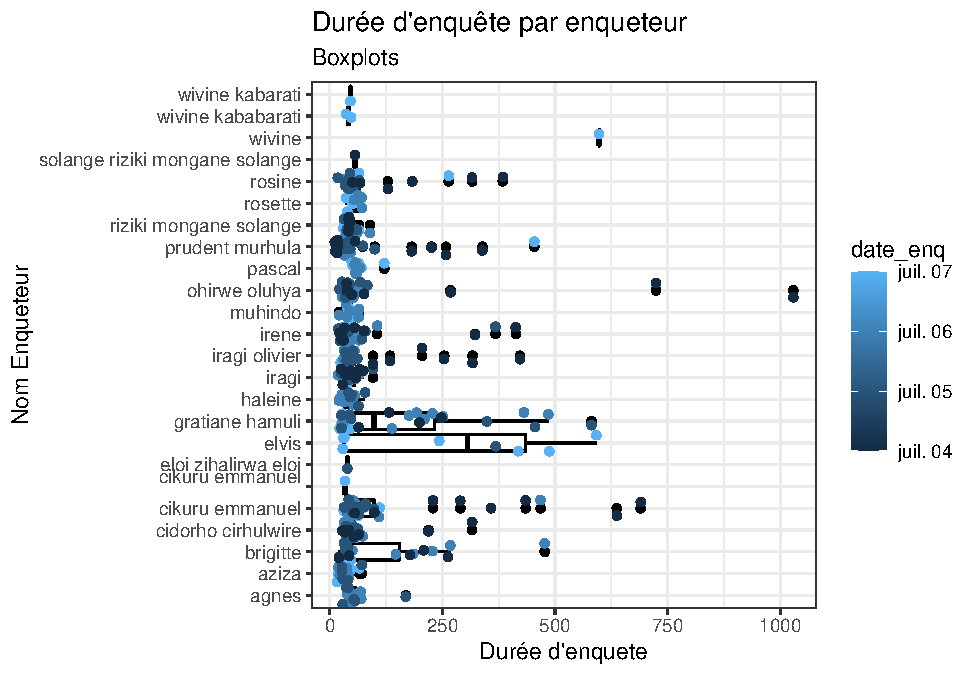
\includegraphics{IES_Endline_SPR_Book_files/figure-latex/unnamed-chunk-15-1.pdf}
De ce graphique, nous remarquons que le temps d'enquête diminue aussi la date avance

\begin{Shaded}
\begin{Highlighting}[]
\FunctionTok{table}\NormalTok{(date\_enq)}
\end{Highlighting}
\end{Shaded}

\begin{verbatim}
## date_enq
## 2021-07-04 2021-07-05 2021-07-06 2021-07-07 2021-07-08 
##         83        112        156        138         38
\end{verbatim}

\begin{Shaded}
\begin{Highlighting}[]
\NormalTok{SPR\_data }\OtherTok{\textless{}{-}}\NormalTok{ SPR\_data }\SpecialCharTok{\%\textgreater{}\%} \FunctionTok{mutate}\NormalTok{(}\AttributeTok{Jour=}\FunctionTok{case\_when}\NormalTok{(date\_enq}\SpecialCharTok{==}\StringTok{"2021{-}07{-}04"}\SpecialCharTok{\textasciitilde{}}\StringTok{"Jour1"}\NormalTok{,}
\NormalTok{                          date\_enq}\SpecialCharTok{==}\StringTok{"2021{-}07{-}05"} \SpecialCharTok{\textasciitilde{}}\StringTok{"Jour2"}\NormalTok{,                                               date\_enq}\SpecialCharTok{==}\StringTok{"2021{-}07{-}07"}\SpecialCharTok{\textasciitilde{}}\StringTok{"Jour3"}\NormalTok{,}
                                               \ConstantTok{TRUE}\SpecialCharTok{\textasciitilde{}}\StringTok{"Jour4"}\NormalTok{))}
\FunctionTok{freq}\NormalTok{(SPR\_data}\SpecialCharTok{$}\NormalTok{Jour,}\AttributeTok{cum=}\NormalTok{T)}
\end{Highlighting}
\end{Shaded}

\begin{verbatim}
##         n    % val%  %cum val%cum
## Jour1  83 15.7 15.7  15.7    15.7
## Jour2 112 21.3 21.3  37.0    37.0
## Jour3 138 26.2 26.2  63.2    63.2
## Jour4 194 36.8 36.8 100.0   100.0
\end{verbatim}

\hypertarget{methodologie}{%
\chapter{Methodologie}\label{methodologie}}

\hypertarget{muxe9thodologie-de-collecte-des-donnuxe9es}{%
\section{Méthodologie de Collecte des Données}\label{muxe9thodologie-de-collecte-des-donnuxe9es}}

\hypertarget{muxe9thodologie-danalyse}{%
\section{Méthodologie d'analyse}\label{muxe9thodologie-danalyse}}

\hypertarget{analyse-des-donnuxe9es}{%
\chapter{Analyse des données}\label{analyse-des-donnuxe9es}}

\hypertarget{description-des-donnuxe9es}{%
\section{Description des Données}\label{description-des-donnuxe9es}}

\hypertarget{construction-des-indicateurs-du-projet}{%
\section{Construction des indicateurs du Projet}\label{construction-des-indicateurs-du-projet}}

\hypertarget{construction-des-indicateurs-de-cohuxe9sion-sociale}{%
\section{Construction des indicateurs de Cohésion Sociale}\label{construction-des-indicateurs-de-cohuxe9sion-sociale}}

\hypertarget{conclusion}{%
\chapter{Conclusion}\label{conclusion}}

  \bibliography{book.bib,packages.bib}

\end{document}
